\documentclass[11pt,a4paper]{article}
\usepackage[margin=2cm]{geometry}
\usepackage{lmodern}
\usepackage[T1]{fontenc}
\usepackage{amsmath,amssymb}
\usepackage{booktabs,array,tabularx,xltabular}
\usepackage{enumitem}
\usepackage{xcolor}
\usepackage[most]{tcolorbox}
\usepackage{titlesec}
\usepackage{graphicx}
\usepackage{float}
\usepackage[font=small,labelfont={bf,color=headblue},skip=4pt]{caption}
\usepackage[colorlinks=true,linkcolor=headblue,urlcolor=blue!50!black]{hyperref}

\definecolor{headblue}{RGB}{38,70,120}
\titleformat{\section}{\Large\bfseries\color{headblue}}{\thesection}{0.8em}{}[{\color{black}\titlerule}]
\titleformat{\subsection}{\large\bfseries\color{headblue}}{\thesubsection}{0.8em}{}
\titleformat{\subsubsection}{\normalsize\bfseries\color{headblue}}{\thesubsubsection}{0.8em}{}
\titlespacing*{\section}{0pt}{12pt}{6pt}
\titlespacing*{\subsection}{0pt}{9pt}{3pt}
\titlespacing*{\subsubsection}{0pt}{7pt}{2pt}
\setlength{\parindent}{0pt}
\setlength{\parskip}{5pt}
\setlist{itemsep=2pt,topsep=2pt}
\setlength{\emergencystretch}{3em}
\renewcommand{\arraystretch}{1.12}
\setlength{\tabcolsep}{4.5pt}
\setlength{\LTpre}{2pt}\setlength{\LTpost}{2pt}
\allowdisplaybreaks
\newtcolorbox{keybox}{colback=blue!3,colframe=headblue!60,boxrule=0.5pt,arc=2mm,left=2mm,right=2mm,top=1mm,bottom=1mm}
\newtcolorbox{insum}{colback=green!3,colframe=green!40!black,boxrule=0.4pt,arc=1.5mm,left=2mm,right=2mm,top=0.5mm,bottom=0.5mm,fontupper=\small}
\newcommand{\inshort}[1]{\begin{insum}\textbf{In short.} #1\end{insum}}
\newcommand{\pct}{\,\%}
\newcommand{\code}[1]{\texttt{#1}}
% title block shared by the three reports: \reporttitle{subtitle}
\newcommand{\reporttitle}[1]{%
\begin{center}
{\LARGE\bfseries\color{headblue} EV Charging with Personal and Commercial Customers\\[2pt] (Formulation 4)}\\[8pt]
{\large #1}\\[6pt]
{\normalsize CP 320 Operations Research for Mobility, course project}\\[2pt]
{\normalsize Yakshith Maddineni (SR 26080) \quad\textperiodcentered\quad Kartikeya Gaur (SR 26371)}\\[2pt]
{\normalsize 27 November 2026}
\end{center}}

\usepackage{adjustbox}
\newcommand{\AgreePers}{82.0}
\newcommand{\AgreeStation}{78.9}
\newcommand{\AgreeType}{93.8}
\newcommand{\AmeComm}{0.0}
\newcommand{\AmePers}{3.2}
\newcommand{\Augment}{8}
\newcommand{\BatchInst}{32}
\newcommand{\BestEpoch}{180}
\newcommand{\BindCC}{22.8}
\newcommand{\BindCP}{9.4}
\newcommand{\BindPC}{35.6}
\newcommand{\BindPP}{17.8}
\newcommand{\BindPoorBehind}{38.5}
\newcommand{\BindPoorOnGun}{23.7}
\newcommand{\BindRichBehind}{6.8}
\newcommand{\BindRichOnGun}{27.8}
\newcommand{\BreakEven}{14}
\newcommand{\CommQShare}{91.2}
\newcommand{\CommShareEV}{70.2}
\newcommand{\CommShareVanFree}{24.2}
\newcommand{\CommUShare}{70.9}
\newcommand{\DeadNZM}{0}
\newcommand{\DeadNZR}{0}
\newcommand{\DeltaOneC}{146}
\newcommand{\DeltaOneP}{-191}
\newcommand{\DeltaOnePDispatch}{1309}
\newcommand{\DeltaZeroC}{393}
\newcommand{\DeltaZeroP}{371}
\newcommand{\DropPenalty}{10}
\newcommand{\ElDiffCoef}{$c^{\mathrm{C,P,1}}$}
\newcommand{\ElDiffM}{8.23}
\newcommand{\ElDiffRL}{9.92}
\newcommand{\ElSumM}{140.2}
\newcommand{\ElSumRL}{139.5}
\newcommand{\ElTopFour}{$c^{\mathrm{C,P,1}}$}
\newcommand{\ElTopFourV}{9.9}
\newcommand{\ElTopOne}{$p^{\mathrm F}$}
\newcommand{\ElTopOneV}{29.3}
\newcommand{\ElTopThree}{$\pi^{\mathrm F}$}
\newcommand{\ElTopThreeV}{16.1}
\newcommand{\ElTopTwo}{$\mu^{\mathrm{C,0}}$}
\newcommand{\ElTopTwoV}{25.7}
\newcommand{\FailedBatches}{0}
\newcommand{\FcsUsersFree}{21\,547}
\newcommand{\FreeVanInst}{2.9}
\newcommand{\GapBestFam}{RC1}
\newcommand{\GapBestFamVal}{0.12}
\newcommand{\GapHundred}{1.02}
\newcommand{\GapMax}{4.79}
\newcommand{\GapMaxN}{90}
\newcommand{\GapMaxNVal}{1.28}
\newcommand{\GapMean}{0.85}
\newcommand{\GapMed}{0.76}
\newcommand{\GapOpt}{0.92}
\newcommand{\GapP}{2.00}
\newcommand{\GapTen}{0.49}
\newcommand{\GapTl}{0.76}
\newcommand{\GapWorstFam}{C2}
\newcommand{\GapWorstFamVal}{1.66}
\newcommand{\GreedyBeat}{353}
\newcommand{\GreedyGap}{-3.33}
\newcommand{\GreedyGapAbs}{3.33}
\newcommand{\GreedyN}{461}
\newcommand{\GreedyWorse}{52}
\newcommand{\GunBindHighR}{85.6}
\newcommand{\GunBindLowR}{2.0}
\newcommand{\GunBindM}{13.5}
\newcommand{\GunBindR}{23.4}
\newcommand{\GunLinksM}{10\,829}
\newcommand{\GunLinksR}{12\,454}
\newcommand{\GunPriceM}{5.1}
\newcommand{\GunPriceMedM}{3.8}
\newcommand{\GunPriceMedR}{4.3}
\newcommand{\GunPriceR}{6.8}
\newcommand{\ImitBatches}{500}
\newcommand{\ImitEpochs}{10}
\newcommand{\InvAfterT}{39}
\newcommand{\InvDroppedMax}{7}
\newcommand{\InvFamOther}{1}
\newcommand{\InvFamR}{31}
\newcommand{\InvFamRC}{28}
\newcommand{\InvHundred}{18}
\newcommand{\InvLone}{49}
\newcommand{\InvLoneNoPlan}{0}
\newcommand{\InvOneEV}{32}
\newcommand{\InvQueue}{13}
\newcommand{\InvSmallestN}{10}
\newcommand{\InvVanBack}{38}
\newcommand{\InvalidInf}{51}
\newcommand{\InvalidNoPlan}{9}
\newcommand{\LPPlansM}{474}
\newcommand{\LPPlansR}{500}
\newcommand{\LPmaxdiffM}{0.0e+00}
\newcommand{\LPmaxdiffR}{0.0e+00}
\newcommand{\LastEpoch}{210}
\newcommand{\LogitAUC}{0.86}
\newcommand{\LogitAcc}{97.3}
\newcommand{\LogitBaseRate}{97.3}
\newcommand{\MILPonly}{0}
\newcommand{\MILPtime}{139.7}
\newcommand{\MILPtimeHundred}{217}
\newcommand{\MILPtotalH}{21.7}
\newcommand{\MilpVanPersKeptRl}{21.0}
\newcommand{\MilpVanPersThetaMean}{0.89}
\newcommand{\MilpVanRlFcs}{1\,037}
\newcommand{\MinEpochs}{200}
\newcommand{\MixMNine}{2.6}
\newcommand{\MixMThree}{14.2}
\newcommand{\MixRLNine}{1.5}
\newcommand{\MixRLThree}{5.0}
\newcommand{\MoneyShareRL}{39.5}
\newcommand{\NEVs}{26\,050}
\newcommand{\NFree}{22\,145}
\newcommand{\NFreeComm}{15\,418}
\newcommand{\NFreePers}{6\,727}
\newcommand{\NInfM}{51}
\newcommand{\NInst}{560}
\newcommand{\NInvalid}{60}
\newcommand{\NNoPlanM}{35}
\newcommand{\NOptM}{277}
\newcommand{\NPaired}{474}
\newcommand{\NPairedOpt}{277}
\newcommand{\NParams}{765\,858}
\newcommand{\NTlM}{197}
\newcommand{\NValid}{500}
\newcommand{\NValidG}{461}
\newcommand{\NValidM}{474}
\newcommand{\OnlyStrandedM}{29.1}
\newcommand{\OnlyStrandedR}{66.5}
\newcommand{\OpShare}{30.8}
\newcommand{\OpShareRL}{29.8}
\newcommand{\PaidKwhComm}{17.1}
\newcommand{\PaidKwhPers}{17.1}
\newcommand{\PatNZM}{0}
\newcommand{\PatNZR}{0}
\newcommand{\Patience}{10}
\newcommand{\PatienceHitR}{0}
\newcommand{\PeakLabelHigh}{38.7}
\newcommand{\PeakLabelLow}{15.6}
\newcommand{\PeakLabelShare}{32.5}
\newcommand{\PerRsPoorComm}{1.84}
\newcommand{\PerRsPoorPers}{1.86}
\newcommand{\PerRsRichComm}{1.82}
\newcommand{\PerRsRichPers}{2.14}
\newcommand{\PercEvComm}{597}
\newcommand{\PercEvMComm}{582}
\newcommand{\PercEvMPers}{662}
\newcommand{\PercEvPers}{699}
\newcommand{\PiC}{0.70}
\newcommand{\PoorQShareComm}{73.2}
\newcommand{\PoorQSharePers}{28.0}
\newcommand{\PoorUShareComm}{61.3}
\newcommand{\PoorUSharePers}{12.6}
\newcommand{\PowerCongM}{7.7}
\newcommand{\PowerCongR}{16.3}
\newcommand{\PowerFM}{432}
\newcommand{\PowerFMedM}{421}
\newcommand{\PowerFMedR}{482}
\newcommand{\PowerFR}{537}
\newcommand{\PowerMM}{67}
\newcommand{\PowerMR}{57}
\newcommand{\PressHi}{0.6897}
\newcommand{\PressHighShareRL}{26.2}
\newcommand{\PressLo}{0.1724}
\newcommand{\PressLong}{0.45}
\newcommand{\PressMax}{2.69}
\newcommand{\PressMedian}{0.310}
\newcommand{\PressNFree}{26\,250}
\newcommand{\PressShareHigh}{32.4}
\newcommand{\PressShareLow}{37.3}
\newcommand{\PressShareMed}{30.3}
\newcommand{\PressShort}{0.64}
\newcommand{\PressWindowMax}{62}
\newcommand{\PressWindowMin}{46}
\newcommand{\QueueMComm}{1.58}
\newcommand{\QueueMPers}{0.41}
\newcommand{\QueueRComm}{3.36}
\newcommand{\QueueRPers}{0.79}
\newcommand{\QueueRPressHigh}{8.78}
\newcommand{\QueueRPressLow}{0.14}
\newcommand{\QueueRPressMedium}{0.90}
\newcommand{\QueueersFcs}{2\,919}
\newcommand{\QueueersM}{7.7}
\newcommand{\QueueersR}{13.5}
\newcommand{\RLbelowOpt}{0}
\newcommand{\RLbetter}{28}
\newcommand{\RLbetterTl}{28}
\newcommand{\RLequal}{54}
\newcommand{\RLequalOpt}{54}
\newcommand{\RLonly}{26}
\newcommand{\RLonlyFams}{C1 1, R1 14, RC1 10, RC2 1}
\newcommand{\RLonlyGr}{39}
\newcommand{\RLonlyMeanN}{85}
\newcommand{\RLtime}{0.119}
\newcommand{\RLtimeHundred}{0.220}
\newcommand{\RLtimeMax}{0.389}
\newcommand{\RLtotalS}{66.8}
\newcommand{\RhoDistVan}{-0.02}
\newcommand{\RhoEPaid}{0.95}
\newcommand{\RhoPressQueue}{0.44}
\newcommand{\RhoSegVan}{-0.16}
\newcommand{\RhoThetaQueue}{-0.15}
\newcommand{\RhoThetaVan}{0.16}
\newcommand{\RlVanMilpFcs}{212}
\newcommand{\Rollouts}{520}
\newcommand{\Samples}{64}
\newcommand{\Speedup}{1\,170}
\newcommand{\SpreadEnd}{1.4}
\newcommand{\StepM}{0.6--0.7}
\newcommand{\StepR}{0.8--0.9}
\newcommand{\StopsM}{4.74}
\newcommand{\StopsR}{4.16}
\newcommand{\StrandedSeatsM}{73.3}
\newcommand{\StrandedSeatsR}{88.0}
\newcommand{\TariffF}{15}
\newcommand{\TariffM}{25}
\newcommand{\TariffShareRL}{38.5}
\newcommand{\TermDFive}{-0.44}
\newcommand{\TermDFour}{-0.23}
\newcommand{\TermDOne}{0.12}
\newcommand{\TermDSix}{2.00}
\newcommand{\TermDThree}{-0.40}
\newcommand{\TermDTwo}{-0.08}
\newcommand{\ThetaFcsR}{0.68}
\newcommand{\ThetaStarP}{0.66}
\newcommand{\ThetaVanComm}{0.34}
\newcommand{\ThetaVanR}{0.85}
\newcommand{\TightBattR}{14.2}
\newcommand{\TightSeatsR}{41.5}
\newcommand{\TightTimeR}{44.3}
\newcommand{\TimeShareRL}{30.7}
\newcommand{\ToChargedHi}{98}
\newcommand{\ToChargedLo}{42}
\newcommand{\TrainMinBest}{33.0}
\newcommand{\TrainMinTotal}{38.6}
\newcommand{\TrainSamples}{8}
\newcommand{\UtilBattM}{71.1}
\newcommand{\UtilBattR}{63.5}
\newcommand{\UtilChargeM}{24.8}
\newcommand{\UtilChargeR}{22.0}
\newcommand{\UtilDepartNeg}{0}
\newcommand{\UtilDriveShareM}{7.6}
\newcommand{\UtilDriveShareR}{8.7}
\newcommand{\UtilFcsShareM}{80.3}
\newcommand{\UtilFcsShareR}{83.5}
\newcommand{\UtilFleetM}{43.9}
\newcommand{\UtilFleetR}{41.6}
\newcommand{\UtilGunHundredM}{14.5}
\newcommand{\UtilGunHundredR}{15.0}
\newcommand{\UtilGunLowFam}{C2}
\newcommand{\UtilGunLowFamV}{3.09}
\newcommand{\UtilGunM}{12.82}
\newcommand{\UtilGunMaxR}{92.4}
\newcommand{\UtilGunR}{13.31}
\newcommand{\UtilGunTopFam}{RC1}
\newcommand{\UtilGunTopFamV}{31.4}
\newcommand{\UtilIdleGunsM}{7.0}
\newcommand{\UtilIdleGunsR}{6.1}
\newcommand{\UtilIdleM}{38.2}
\newcommand{\UtilIdleR}{41.6}
\newcommand{\UtilKwhInst}{987}
\newcommand{\UtilLossShareR}{9.1}
\newcommand{\UtilPaired}{474}
\newcommand{\UtilPeakGunsM}{12.9}
\newcommand{\UtilPeakGunsMaxM}{24}
\newcommand{\UtilPeakGunsMaxR}{24}
\newcommand{\UtilPeakGunsR}{13.1}
\newcommand{\UtilProfPeakAt}{0.03}
\newcommand{\UtilProfPeakM}{24.7}
\newcommand{\UtilProfPeakR}{24.7}
\newcommand{\UtilRoadM}{68.4}
\newcommand{\UtilRoadR}{68.6}
\newcommand{\UtilSeatM}{79.0}
\newcommand{\UtilSeatR}{69.4}
\newcommand{\UtilSysM}{12.39}
\newcommand{\UtilSysR}{12.39}
\newcommand{\UtilVanKwhM}{88.7}
\newcommand{\UtilVanKwhR}{78.2}
\newcommand{\UtilVanKwhTotM}{92\,205}
\newcommand{\UtilVanKwhTotR}{77\,076}
\newcommand{\UtilVansM}{1\,040}
\newcommand{\UtilVansR}{985}
\newcommand{\ValBest}{0.969}
\newcommand{\ValBestFifty}{0.980}
\newcommand{\ValBestHundred}{0.927}
\newcommand{\ValBestPct}{3.1}
\newcommand{\ValBestTwenty}{1.001}
\newcommand{\ValFirstRf}{1.007}
\newcommand{\ValImitEnd}{1.023}
\newcommand{\ValStart}{3.57}
\newcommand{\ValUnplGr}{2.99}
\newcommand{\ValUnplRl}{2.30}
\newcommand{\ValUnplStart}{28.9}
\newcommand{\ValidRCone}{52}
\newcommand{\ValidRone}{89}
\newcommand{\VanBindM}{38.7}
\newcommand{\VanBindR}{41.5}
\newcommand{\VanCommPressHigh}{3.6}
\newcommand{\VanCommPressLow}{0.0}
\newcommand{\VanCommPressMedium}{0.0}
\newcommand{\VanLowRComm}{1.1}
\newcommand{\VanLowRPers}{0.0}
\newcommand{\VanMAll}{6.5}
\newcommand{\VanMComm}{0.7}
\newcommand{\VanMPers}{19.9}
\newcommand{\VanPersPressHigh}{4.4}
\newcommand{\VanPersPressLow}{9.4}
\newcommand{\VanPersPressMedium}{5.1}
\newcommand{\VanPriceM}{5.51}
\newcommand{\VanPriceR}{5.47}
\newcommand{\VanRAll}{2.7}
\newcommand{\VanRComm}{0.9}
\newcommand{\VanRPers}{6.7}
\newcommand{\VanShareEV}{17.6}
\newcommand{\VanTopLong}{12.9}
\newcommand{\VanTopMComm}{0.0}
\newcommand{\VanTopMPers}{40.8}
\newcommand{\VanTopRComm}{0.0}
\newcommand{\VanTopRPers}{12.7}
\newcommand{\VanTopShort}{12.4}
\newcommand{\VanWaitZero}{51.5}
\newcommand{\VansFullM}{48.1}
\newcommand{\VansFullR}{19.4}
\newcommand{\VansM}{1\,040}
\newcommand{\VansMean}{2.2}
\newcommand{\VansR}{985}
\newcommand{\ZevMax}{1132}
\newcommand{\ZevMean}{898}
\newcommand{\ZevMin}{776}


\begin{document}

\reporttitle{Comprehensive RL report: method, training, exploratory analysis and behaviour}

\begin{keybox}
{\color{headblue}\textbf{How to read this report}}\\
The reinforcement-learning (RL) method of formulation 4: an attention network, trained with REINFORCE, that builds a plan one decision at a time. \textbf{Part I}: method and every assumption. \textbf{Part II}: training and an exploratory analysis of the \NInst{} RL runs. \textbf{Part III}: the results point by point, from quality and feasibility to shadow prices, infrastructure utilisation, equity and why RL behaves as it does. The MILP appears where it explains the RL; the full comparison is in the results report. Green \emph{In short} boxes close every subsection; Section~\ref{sec:glossary} explains every term.
\end{keybox}

\begin{keybox}
{\color{headblue}\textbf{The main results in eleven lines}}
\begin{enumerate}[leftmargin=1.4em,itemsep=1pt]
  \item RL gives a valid plan for \NValid{} of \NInst{} instances, the MILP for \NValidM. RL has a plan for \RLonly{} instances where the MILP found none in 300\,s, and never misses one the MILP has (Section~\ref{sec:feasibility}).
  \item All \NInvalid{} invalid RL plans are instances the MILP could not solve either. \InvalidInf{} are proven infeasible, and in \InvLone{} of them one car cannot be charged by $T$ even alone (Section~\ref{sec:feasibility}).
  \item Where both have a plan, RL costs \GapMean\pct{} more than the MILP (median \GapMed\pct). Against proven optima the gap is \GapOpt\pct; RL matches the optimum in \RLequalOpt{} instances and beats the MILP's time-limit plan in \RLbetter{} (Section~\ref{sec:quality}).
  \item RL beats the greedy rule it was warm-started from in \GreedyBeat{} of \GreedyN{} instances and is \GreedyGapAbs\pct{} cheaper on average (Section~\ref{sec:quality}).
  \item RL needs \RLtime\,s per instance against \MILPtime\,s for the MILP, about \Speedup{} times faster. Its \TrainMinBest{} minutes of training pay off after about \BreakEven{} instances (Section~\ref{sec:compute}).
  \item The extra cost is almost entirely customer time ($Z_6$: +\TermDSix{} points of $Z$). It is partly offset by lower tariff, dispatch and energy costs, because RL serves fewer customers by van (Section~\ref{sec:anatomy}).
  \item Segment and income still decide who gets a van, as the theory says: in RL plans personal cars get vans (\VanRPers\pct) and commercial cars almost never do (\VanRComm\pct). The personal step comes later, at $\theta$ \StepR{} against \StepM{} in the MILP and $\theta^{*}=\ThetaStarP$ in theory (Section~\ref{sec:income}).
  \item On the instances both solve, RL dispatches slightly fewer vans than the MILP (\VansR{} against \VansM) and fills them less: \VansFullR\pct{} of its vans are full against \VansFullM\pct, and \OnlyStrandedR\pct{} serve only stranded cars (Section~\ref{sec:util}).
  \item The infrastructure is lightly used by both methods: a gun is busy \UtilGunR\pct{} of the planning period in RL plans (MILP \UtilGunM\pct) and \UtilIdleGunsR{} of 24 guns stay idle per instance. RL charges \UtilFcsShareR\pct{} of the energy at stations (MILP \UtilFcsShareM\pct), and its vans deliver \UtilVanKwhR{} kWh each against \UtilVanKwhM{} (Section~\ref{sec:util}).
  \item Shadow prices show the consequence. Gun-minutes are scarce more often in RL plans (\GunBindR\pct{} of gun links binding against \GunBindM\pct), commercial queues are longer (\QueueRComm{} against \QueueMComm{} min), and one more kW at the stations is worth more (\PowerFR{} against \PowerFM{} Rs per instance; Section~\ref{sec:duals}).
  \item The cost structure, the elasticities and the zero value of patience limits and the deadline are the same as for the MILP (Sections~\ref{sec:anatomy}, \ref{sec:duals}).
\end{enumerate}
\end{keybox}

\newpage
\tableofcontents
\newpage

%=====================================================================
\section{Glossary}
\label{sec:glossary}

\begin{xltabular}{\textwidth}{@{}>{\raggedright\arraybackslash}p{4.0cm}X@{}}
\toprule
\textbf{Term} & \textbf{Meaning} \\
\midrule
\endhead
\multicolumn{2}{@{}l}{\textit{The problem (shared with the MILP)}} \\
EV, FCS, gun, van & Electric vehicle; fixed charging station with 2 guns of 22\,kW; mobile charging van (150\,kWh, 30\,kW, at most 6 EVs, starts and ends at the depot). \\
Request time $r_i$, horizon $T$ & Minute EV $i$ asks for charging; length of the planning period. Every EV must be fully charged and every van back by $T$. \\
Stranded / free-choice EV & Stranded: no station within range, so only a van can serve it. Free-choice: at least one station in range. \\
Segment $s_i$ & Personal (private owner, driver free while a van charges the parked car) or commercial (taxi or fleet car: every minute out of service is lost income). Commercial with probability $\pi_{\mathrm C}=\PiC$. \\
Income index $\theta_i$ & Owner's income in $[0,1]$. Personal $\theta\sim$ Beta(2.5,\,1), commercial $\theta\sim$ Beta(3,\,5). \\
$\mu$, $c^{a}$, $W$ & Money sensitivity, value of time in activity $a$ (D driving, Q queueing, C charging at a station, V van wait and charging), queue tolerance; straight lines in $\theta$ with their own end points per segment. \\
Downtime rate $\omega$ & For a commercial car $c^{\mathrm D}=c^{\mathrm C}=c^{\mathrm V}=\omega(\theta)$: one price for every minute out of service. \\
Tariff $p^{\mathrm F}$, $p^{\mathrm M}$ & Price per kWh the customer pays at a station (\TariffF{} Rs) and for the van (\TariffM{} Rs). \\
Objective $Z$ & Operator cost ($Z_2$--$Z_4$) plus perceived customer cost ($Z_1$, $Z_5$, $Z_6$). \\
MILP & The exact model, solved by Gurobi with a 300\,s limit; the benchmark here. \\
Optimal / time-limit plan & MILP plan proven optimal / found when the time ran out (not proven optimal). \\
Infeasible & No plan can meet all constraints; proven by Gurobi. \\
Greedy rule & The rule that builds a plan EV by EV, choosing each time the option with the smallest increase of $Z$ (the MILP's warm start). \\
Valid / invalid plan & A plan that meets every constraint / one that breaks at least one, as judged by the independent checker. \\
Gap & $100\,(Z_{\mathrm{RL}}-Z_{\mathrm{other}})/Z_{\mathrm{other}}$ over instances where both plans are valid; negative means RL is cheaper. \\
\multicolumn{2}{@{}l}{\textit{Reinforcement learning}} \\
Reinforcement learning (RL) & Learning a decision rule by trial and error from a reward signal, instead of solving each instance from scratch. \\
Markov decision process (MDP) & The problem written as a sequence of decisions: a \emph{state} (what has been placed so far), an \emph{action} (the next decision) and a \emph{reward} (minus the increase of $Z$). \\
State & Which EVs are placed; for each gun the minute it becomes free; for each van its position, the minute it is free, battery left and EVs served. \\
Action & A pair (EV $i$, resource $k$): EV $i$ is appended to the queue of gun $k$ or to the route of van $k$. \\
Episode, rollout & One complete construction of a plan, decision by decision. \\
Policy $\pi$ & The decision rule: a probability for every possible action in every state. Here a neural network. \\
Embedding & A vector of numbers that represents a node (EV, station, depot) inside the network. \\
Attention, Transformer & A network layer in which every node looks at every other node and weighs them; a Transformer stacks such layers. \\
Encoder / decoder & Encoder: turns the whole instance into embeddings once. Decoder: picks one action at a time from them. \\
Pointer network & A decoder that chooses an item of its input (here an EV, then a gun or a van) by scoring each item. \\
Mask & Removes infeasible actions before the choice, so only feasible (EV, resource) pairs can be picked. \\
Greedy vs sampled rollout & Greedy: always take the most probable action. Sampled: draw actions at random from $\pi$. \\
REINFORCE, policy gradient & Training rule: make the actions of cheap rollouts more likely and those of expensive rollouts less likely. \\
Baseline, advantage & Baseline: a reference cost; advantage: how much cheaper a rollout was than the baseline. \\
Shared (POMO) baseline & The baseline of an instance is the mean cost of all its rollouts in the batch. \\
Imitation warm-up, teacher forcing & First phase of training, in which the network learns to copy the greedy rule's choices before REINFORCE. \\
Batch, epoch & Batch: one training step on a group of random instances. Epoch: \(50\) batches followed by a validation. \\
Learning rate & Step size of the parameter updates. \\
Validation ratio & Cost of the network's greedy rollout divided by the cost of the greedy rule, on fixed validation instances; below 1 means better than the rule. \\
Early stopping & Stop training when the validation ratio has not improved for a number of epochs. \\
Training generator & Code that makes new random training instances with the dataset's rules; the 56 test files are never used in training. \\
Map symmetries (augmentation) & Rotating or reflecting the map gives 8 versions of the same instance with different network inputs. \\
Zero-shot & Using a trained network on inputs it was not trained for (other parameters, fleet or files) without retraining. \\
Inference & Using the trained network to solve a new instance. \\
Unplaced EV & EV for which no feasible action is left during a rollout; the plan is then invalid. \\
\multicolumn{2}{@{}l}{\textit{Analysis (as in the MILP report)}} \\
Shadow price, fixed-plan LP & Dual value of a constraint after fixing a plan's yes/no decisions and re-solving the timing LP. \\
Binding constraint & Constraint that holds with equality; only binding constraints can have a non-zero shadow price. \\
Envelope theorem, elasticity & $\partial Z/\partial c_k$ = the quantity $c_k$ multiplies; elasticity = share of $Z$ carried by $c_k$. \\
Demand pressure & How busy the system is when EV $i$ asks: the number of requests of the instance released during one mean station charging time up to and including $r_i$, divided by the 29 chargers (24 guns and 5 vans). Data only; one definition and one set of terciles for all three reports (Section~\ref{sec:defs}). \\
Peak / off-peak (formulation 4 label) & Coarser label of the formulation-4 code: peak if an EV's load exceeds the median load of its instance. Not used for the terciles here. \\
Utilisation & Share of the planning period $[0,T]$ a gun or van is charging (= share of its energy capacity used, at constant power); seats, battery and time used by a van (Section~\ref{sec:util}). \\
Wilson interval & 95\,\% confidence interval for a share; reliable for small or extreme shares. \\
Logistic regression, AME & Model of the probability of a yes/no outcome; average marginal effect = average change of that probability per unit of a factor. \\
AUC & Probability that the model ranks a random van user above a random station user (0.5 = no better than chance). \\
Spearman correlation & Correlation of the ranks of two variables, from $-1$ to $+1$. \\
Solomon family & C (clustered), R (random), RC (mixed); type 1 short horizon, type 2 long horizon. \\
\bottomrule
\end{xltabular}

%=====================================================================
\clearpage
\part{Method and assumptions}

\section{All assumptions behind the RL results}
\label{sec:assumptions}

\subsection{The problem in one paragraph}
During a planning period $[0,T]$ parked EVs request charging. Each request is served by exactly one resource: the EV drives to a station and charges at one of its guns, or a van drives to the EV and charges it in place. A plan says who is served where, the order on every gun, the route of every van and every start time. It minimises the operator's cost plus the cost each customer perceives. Every customer weighs money and time according to a use segment (personal or commercial) and an income index $\theta_i$. This is formulation 4 (\code{formulation\_4.pdf}, equations (1)--(23)). The RL method solves exactly this problem; only the way of finding a plan differs from the MILP.

\subsection{Assumptions shared with the MILP}
The RL plans are scored by the same independent checker (\code{check\_plan\_f4.py}) as the MILP plans and use the same data (\NInst{} instances: 56 Solomon files, first $n=10,20,\dots,100$ EVs). All modelling assumptions of the MILP hold:
\begin{itemize}
  \item offline planning (all requests known at time 0);
  \item every EV fully charged by $T$, and every van back at the depot by $T$;
  \item stations within range only;
  \item one EV per gun and per van at a time;
  \item constant charging power;
  \item van energy for driving and charging from one battery;
  \item customer coefficients fixed by segment and income.
\end{itemize}
The customer parameters are in Table~\ref{tab:params}; the network, fleet and cost data are those of the MILP report.

\begin{table}[H]\centering\small
\caption{Customer parameters of the run (straight lines between $\theta=0$ and $\theta=1$, per segment). Commercial: $c^{\mathrm D}=c^{\mathrm C}=c^{\mathrm V}=\omega$.}\label{tab:params}
\begin{adjustbox}{max width=\textwidth}\begin{tabular}{llrrrr}\toprule
parameter & unit & pers. $\theta=0$ & pers. $\theta=1$ & comm. $\theta=0$ & comm. $\theta=1$ \\ \midrule
income $\theta$ & -- & \multicolumn{2}{c}{Beta(2.5, 1)} & \multicolumn{2}{c}{Beta(3, 5)} \\
money sensitivity $\mu$ & Rs/Rs & 1.5 & 0.5 & 1.5 & 0.5 \\
value of time $c^{\mathrm D}$ (driving) & Rs/min & 1.5 & 15 & 1.5 & 6 \\
value of time $c^{\mathrm Q}$ (queueing) & Rs/min & 2.5 & 25 & 2 & 7.5 \\
value of time $c^{\mathrm C}$ (FCS charging) & Rs/min & 1 & 10 & 1.5 & 6 \\
value of time $c^{\mathrm V}$ (van wait + charging) & Rs/min & 0.5 & 5 & 1.5 & 6 \\
queue tolerance $W$ & min & 60 & 15 & 40 & 15 \\
\bottomrule\end{tabular}\end{adjustbox}

\end{table}

\subsection{Assumptions of the learning method}
\begin{xltabular}{\textwidth}{@{}>{\raggedright\arraybackslash}p{4.4cm}>{\raggedright\arraybackslash}p{4.4cm}X@{}}
\toprule
\textbf{Assumption} & \textbf{Why} & \textbf{What changes if relaxed} \\
\midrule
\endhead
The plan is built one (EV, resource) pair at a time; each EV is appended to the end of a gun queue or van route. & Turns the problem into an MDP that a network can learn. & Inserting EVs anywhere in a sequence would allow better orders but makes actions and masks more complex. \\
Start times are not learned: every session starts as early as possible. & With assignments and orders fixed, every time cost grows with a later start, so earliest start is optimal (checked exactly by the fixed-plan LPs, Section~\ref{sec:duals}). & Nothing would be gained. \\
Masks enforce range, queue limit $W_i$, deadline $T$, van seats, battery and return by $T$ at every step. & Only feasible plans can be built while EVs remain placeable. & Without masks the network would have to learn feasibility from penalties. \\
An EV with no feasible action left is dropped and later appended where it finishes earliest; the plan is then invalid. & Every instance gets a complete plan that the checker can judge. & A repair heuristic could fix some plans, but would no longer be the policy's own result. \\
Reward = minus the increase of $Z$ caused by the action, with the same six terms as the checker. & The rewards add up exactly to $-Z$. & -- \\
Training on new random instances made with the dataset's rules; the 56 test files are never seen in training. & Tests generalisation honestly. & Training on the test files would overstate quality. \\
Segment, $\mu$ and the cost of queueing one charging time ($c^{\mathrm Q}\tau^{\mathrm F}$) are extra EV inputs. & The policy must see what makes customers differ in formulation 4. & Without them it could not treat personal and commercial cars differently. \\
Warm-up by imitating the greedy rule, then REINFORCE with a shared baseline. & A sensible starting policy; low-variance gradient. & Pure RL from random weights starts with \ValUnplStart\pct{} unplaced EVs. \\
Best of \Rollouts{} rollouts per instance (\Augment{} symmetries $\times$ (1 greedy + \Samples{} sampled)). & Cheap search at inference time. & Fewer rollouts: faster, slightly worse plans. \\
\bottomrule
\end{xltabular}

\subsection{Network, training and inference}
\textbf{Network.} The network has \NParams{} parameters. It does not receive the demand pressure of Section~\ref{sec:defs}; congestion reaches it only through the gun and van free times, the EV's rank among the open requests and the cost of its cheapest options. An attention encoder (Kool et al.\ 2019) embeds every EV, station and the depot. EV features include position, energy, request time, range, segment, $\mu$ and the cost of a queue. A two-step pointer decoder first scores the open EVs, then scores the resources for the chosen EV: every gun, and every van at its current position. Scores combine attention with small networks on dynamic features (options left, cheapest option, regret, earliest finish, free times, battery). Masked actions get probability 0; $\log\pi(\text{action})=\log\pi(i)+\log\pi(k\mid i)$.

\textbf{Training.} Training starts with \ImitBatches{} warm-up batches (\ImitEpochs{} epochs) that teach the greedy rule's actions. Then comes REINFORCE: each batch has \BatchInst{} random instances of one size $n\in[10,100]$, each rolled out \TrainSamples{} times. The advantage is the rollout's cost relative to the mean of its instance, and each unplaced EV adds \DropPenalty{} instance cost scales. After every epoch the network's greedy rollout is compared with the greedy rule on fixed validation instances. The best epoch is kept; at least \MinEpochs{} epochs always run, and training stops after \Patience{} epochs without improvement.

\textbf{Inference.} The best of \Rollouts{} rollouts per instance is kept (fewest unplaced EVs, then lowest $Z$) and scored by the checker. No repair is applied.

\begin{table}[H]\centering\small
\caption{Network, training, inference and hardware settings (\code{rl\_f4\_params.json}, \code{train\_meta.json}, \code{meta.json}).}\label{tab:settings}
\begin{adjustbox}{max width=\textwidth}\begin{tabular}{llr}\toprule
 & setting & value \\ \midrule
Network & embedding size $d$ / heads / encoder layers & 128 / 8 / 3 \\
 & feed-forward width / logit clip $C$ / dynamic MLP width & 512 / 10 / 32 \\
 & trainable parameters & 765\,858 \\
Generator & templates (file size, class) & 6 (100 EVs; C1 \dots RC2) \\
 & clusters / cluster spread (share of area) & 5--12 / 0.015--0.05 \\
 & share of requests at $t=0$ / Beta shape of the rest & 0.15--0.3 / $a\in[1.0,2.5]$ \\
 & latest request (share of $T$) / jitter of $T$ & 0.83--0.92 / $\pm15$\% \\
Training & imitation warm-up batches / learning rate & 500 / 0.0001 \\
 & REINFORCE learning rate / decay per epoch & 2e-05 / 0.9998 \\
 & instances per batch $\times$ rollouts per instance & 32 $\times$ 8 \\
 & batches per epoch / instance size $n$ & 50 / 10--100 \\
 & penalty per unplaced EV (cost scales) & 10 \\
 & stop rule & $\ge$200 epochs, patience 10, max 500, 8 h \\
 & validation & 24 instances at $n\in\{20,50,100\}$ \\
Inference & map symmetries $\times$ (greedy + sampled rollouts) & 8 $\times$ (1 + 64) = 520 \\
 & plan kept & fewest unplaced EVs, then lowest $Z$ \\
Hardware & device / CPU threads / torch & CUDA GPU / 24 / 2.14.1 \\
\bottomrule\end{tabular}\end{adjustbox}

\end{table}

\subsection{Evaluation and analysis definitions}
\label{sec:defs}
\begin{itemize}
  \item The MILP benchmark is the run \code{milp\_300s} (Gurobi 13, 300\,s, 4 threads per instance); the greedy rule is the run \code{greedy}. Both are on the same \NInst{} instances.
  \item Shares of ``served by a van'' are over free-choice EVs only; stranded EVs take a van whatever their segment and income.
  \item \textbf{Demand pressure} (the same definition, computed by the same code \code{common/infra.py}, in all three reports). For EV $i$ of an instance:
  \begin{gather*}\text{window}=\frac1n\sum_{j}\frac{60E_j}{22\text{ kW}},\qquad \text{load}_i=\#\{j:\ r_i-\text{window}\le r_j\le r_i\}\ \ (i\text{ included}),\\ \text{pressure}_i=\frac{\text{load}_i}{24\text{ guns}+5\text{ vans}} .\end{gather*}
  The window is the mean station charging time of the instance's EVs (\PressWindowMin--\PressWindowMax{} minutes). Pressure uses only the data, never a plan, so an EV has the same pressure for RL and MILP. Terciles are pooled over the \PressNFree{} free-choice EVs of all \NInst{} baseline instances: low $\le\PressLo<$ medium $\le\PressHi<$ high (\PressShareLow\pct, \PressShareMed\pct{} and \PressShareHigh\pct{} of them; the shares are not equal because many EVs share the same load).
  It ignores travel time to the station, charging still in progress from earlier requests and the difference between a gun and a van (a van counts as one charger). The formulation-4 code also labels an EV ``peak'' when its load exceeds the median load of its instance; that label is coarser and instance-relative (\PeakLabelShare\pct{} of free-choice EVs are ``peak'', of which only \PeakLabelHigh\pct{} are in the high tercile) and is not used here.
  \item \textbf{The policy does not see demand pressure.} The network receives no pressure input. What it does receive and is related: each EV's request time relative to $T$ and to the earliest open request, its rank among the open requests, the free time of every gun and van, the earliest finish over its feasible options, and the cost of its cheapest options (which grows with the queue it would face).
  \item \textbf{Utilisation} is computed from each plan by \code{common/infra.py} (Section~\ref{sec:util}): gun time over $[0,T]$, van seats, battery, time and energy, and the system's installed capacity.
  \item Shadow prices come from the fixed-plan LP of every valid plan, RL and MILP alike (Section~\ref{sec:duals}).
\end{itemize}

\inshort{RL solves formulation 4 exactly as stated: same constraints, same objective, same checker as the MILP. What is learned is the order of decisions and the choice of resource; timing is computed exactly, and masks keep every step feasible.}

%=====================================================================
\clearpage
\part{Training and exploratory analysis}

\section{Training}
\label{sec:training}

\begin{figure}[H]
\centering
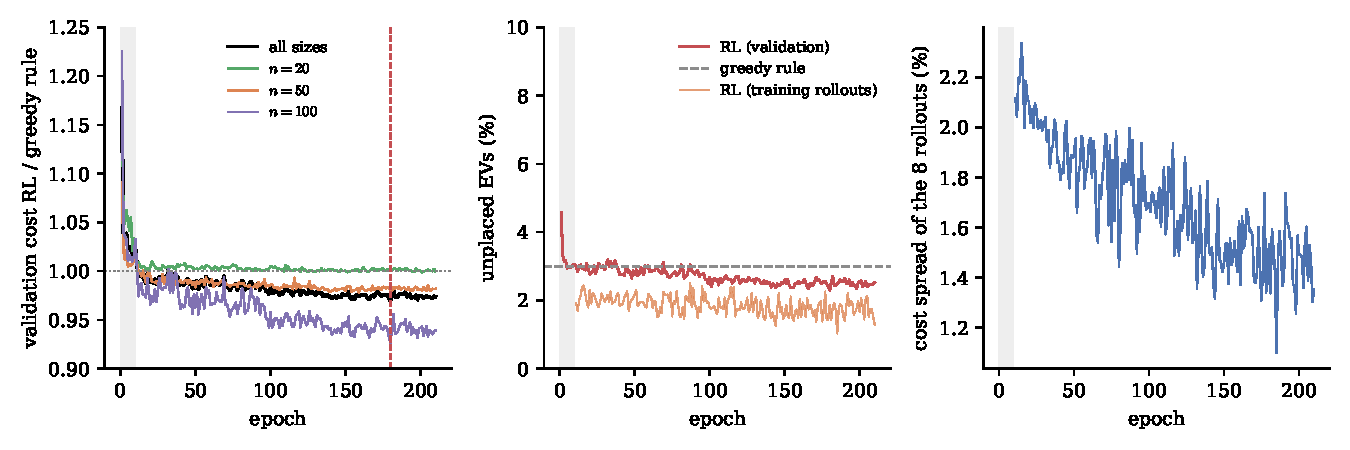
\includegraphics[width=\textwidth]{figures/r_training.pdf}
\caption{Left: validation cost of the network's greedy rollout relative to the greedy rule (black: all sizes; dashed red line: best epoch). Middle: unplaced EVs. Right: spread of the 8 rollout costs of an instance during training. Grey band: imitation warm-up.}
\label{fig:training}
\end{figure}

\begin{itemize}
  \item \textbf{Warm-up.} The untrained network costs \ValStart{} times the greedy rule on the validation instances and leaves \ValUnplStart\pct{} of EVs unplaced. After the \ImitEpochs{} imitation epochs it is close to the rule (ratio \ValImitEnd).
  \item \textbf{REINFORCE.} The ratio falls below 1 and reaches its best, \ValBest, at epoch \BestEpoch: on the validation instances the network is \ValBestPct\pct{} cheaper than the rule it learned from. By size the ratio is \ValBestTwenty{} at $n=20$, \ValBestFifty{} at $n=50$ and \ValBestHundred{} at $n=100$; the larger the instance, the more there is to gain over a myopic rule.
  \item \textbf{Feasibility.} At the best epoch the network leaves \ValUnplRl\pct{} of validation EVs unplaced, against \ValUnplGr\pct{} for the greedy rule.
  \item \textbf{Stop.} Training stopped early at epoch \LastEpoch{}, after \Patience{} epochs without improvement, \TrainMinTotal{} minutes in all (best model after \TrainMinBest{} minutes). No batch failed (\FailedBatches). The spread of the 8 rollouts of an instance settles at about \SpreadEnd\pct: the policy has become nearly deterministic.
\end{itemize}

\inshort{Training is short (\TrainMinTotal{} minutes on one GPU) and stable. The network starts from the greedy rule, ends \ValBestPct\pct{} cheaper than it on validation instances, and gains most on large instances.}

\clearpage
\section{Exploratory analysis of the RL results}
\label{sec:explore}

\subsection{How the instances ended}
\begin{figure}[H]
\centering
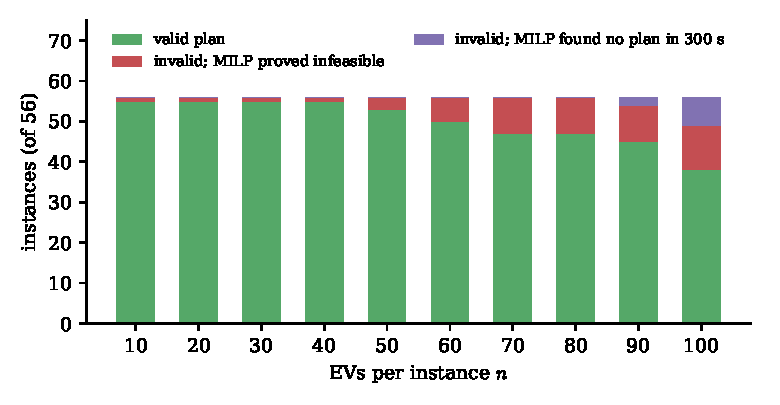
\includegraphics[width=0.62\textwidth]{figures/r_outcome.pdf}
\caption{Outcome of the 56 instances of each size, with the MILP's verdict on the invalid ones.}
\label{fig:outcome}
\end{figure}

\begin{table}[H]\centering
\caption{RL outcome per instance size, next to the MILP (300\,s) and the greedy rule. RL only = RL has a valid plan, the MILP none.}\label{tab:outcome}
\begin{adjustbox}{max width=\textwidth}\begin{tabular}{lrrrrrrr}\toprule
$n$ & instances & RL valid & RL invalid & MILP plan & greedy plan & RL only & RL time (s) \\ \midrule
10 & 56 & 55 & 1 & 55 & 55 & 0 & 0.030 \\
20 & 56 & 55 & 1 & 55 & 55 & 0 & 0.044 \\
30 & 56 & 55 & 1 & 55 & 55 & 0 & 0.064 \\
40 & 56 & 55 & 1 & 55 & 53 & 0 & 0.085 \\
50 & 56 & 53 & 3 & 53 & 48 & 0 & 0.106 \\
60 & 56 & 50 & 6 & 49 & 45 & 1 & 0.127 \\
70 & 56 & 47 & 9 & 44 & 43 & 3 & 0.149 \\
80 & 56 & 47 & 9 & 39 & 38 & 8 & 0.172 \\
90 & 56 & 45 & 11 & 36 & 36 & 9 & 0.195 \\
100 & 56 & 38 & 18 & 33 & 33 & 5 & 0.220 \\
\midrule all & 560 & 500 & 60 & 474 & 461 & 26 & 0.119 \\
\bottomrule\end{tabular}\end{adjustbox}\end{table}

\begin{table}[H]\centering
\caption{RL outcome against the MILP outcome of the same instance.}\label{tab:crosstab}
\begin{adjustbox}{max width=\textwidth}\begin{tabular}{lrrrrr}\toprule
RL $\backslash$ MILP & optimal & time limit, plan & time limit, no plan & infeasible & total \\ \midrule
valid plan & 277 & 197 & 26 & 0 & 500 \\
invalid plan & 0 & 0 & 9 & 51 & 60 \\
\bottomrule\end{tabular}\end{adjustbox}\end{table}


RL has a valid plan in \NValid{} instances, the MILP in \NValidM{} and the greedy rule in \NValidG. Every instance the MILP solved, RL solved too (\MILPonly{} exceptions), and RL also has plans for \RLonly{} instances where the MILP found none in 300\,s. The \NInvalid{} invalid RL plans are the \InvalidInf{} instances the MILP proved infeasible plus \InvalidNoPlan{} where the MILP found no plan either. Invalid plans start at $n=\InvSmallestN$ and are most frequent at $n=100$ (\InvHundred).

\inshort{\NValid{} valid plans; RL fails only where the MILP fails too.}

\subsection{Instance-level overview}
\begin{table}[H]\centering
\small
\caption{Distribution of instance-level results over the valid RL plans.}\label{tab:inststats}
\begin{adjustbox}{max width=\textwidth}\begin{tabular}{lrrrrrrr}\toprule
measure (per instance) & count & mean & median & 10th pct & 90th pct & min & max \\ \midrule
objective $Z$ per EV (Rs) & 500 & 898 & 875 & 813 & 1027 & 776 & 1132 \\
operator share of $Z$ (\%) & 500 & 30.8 & 30.0 & 27.5 & 37.4 & 18.9 & 48.0 \\
vans used & 500 & 2.2 & 2.0 & 1.0 & 4.0 & 0.0 & 5.0 \\
EVs served by a van (\%) & 500 & 17.6 & 16.7 & 12.0 & 25.0 & 0.0 & 40.0 \\
free-choice EVs by van (\%) & 500 & 2.9 & 1.2 & 0.0 & 7.4 & 0.0 & 22.2 \\
mean FCS queue (min) & 500 & 1.88 & 0.19 & 0.00 & 7.82 & 0.00 & 15.12 \\
mean van wait (min) & 493 & 22.3 & 14.9 & 0.0 & 53.0 & 0.0 & 147.3 \\
mean request to charged (min) & 500 & 64.8 & 60.8 & 55.0 & 79.5 & 48.5 & 111.9 \\
van km & 500 & 71.0 & 69.1 & 21.6 & 127.1 & 0.0 & 240.1 \\
RL time (s), all instances & 560 & 0.119 & 0.119 & 0.042 & 0.201 & 0.023 & 0.389 \\
\bottomrule\end{tabular}\end{adjustbox}\end{table}


\begin{figure}[H]
\centering
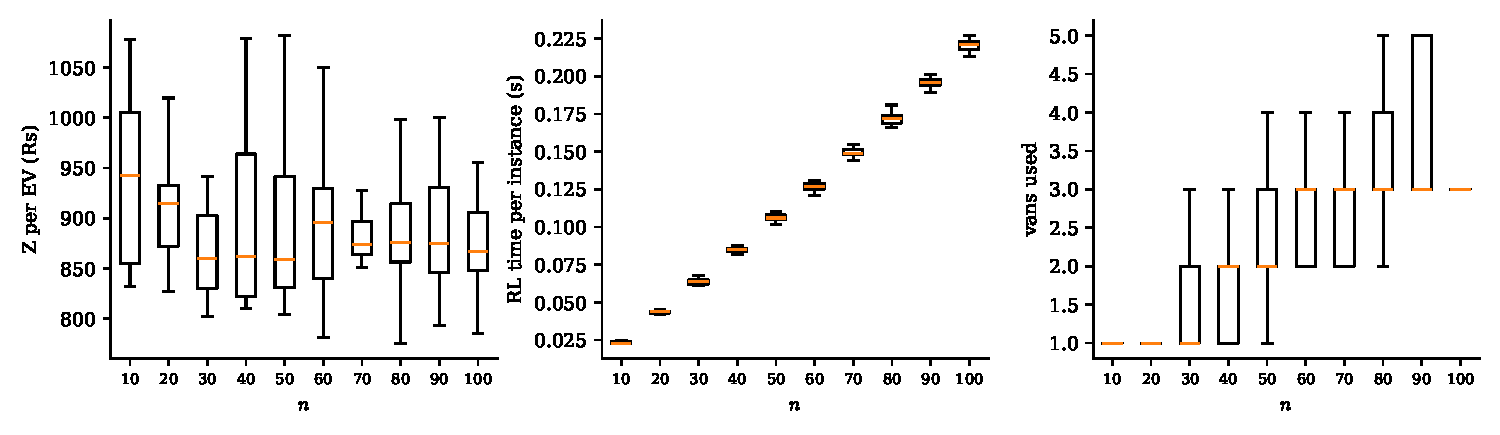
\includegraphics[width=0.95\textwidth]{figures/r_inst_by_n.pdf}
\caption{Objective per EV, RL time and vans used by instance size (boxes: middle 50\,\%).}
\label{fig:instbyn}
\end{figure}

\begin{itemize}
  \item The objective per EV is \ZevMean{} Rs on average (between \ZevMin{} and \ZevMax). About \OpShare\pct{} of it is operator cost.
  \item About \VansMean{} vans leave per instance and serve \VanShareEV\pct{} of the EVs, mostly the stranded ones. Only \FreeVanInst\pct{} of free-choice EVs per instance get a van.
  \item RL time grows with $n$ but stays below half a second (\RLtimeMax\,s at most).
\end{itemize}

\subsection{Families}
\begin{table}[H]\centering
\small
\caption{RL results by Solomon family (valid plans).}\label{tab:family}
\begin{adjustbox}{max width=\textwidth}\begin{tabular}{lrrrrrrrrr}\toprule
family & instances & valid & $Z$/EV (Rs) & operator (\%) & free-choice by van (\%) & queue (min) & to charged (min) & vans & $T$ (min) \\ \midrule
C1 & 90 & 90 & 878 & 30.8 & 3.8 & 0.89 & 61.1 & 2.16 & 1236 \\
C2 & 80 & 79 & 897 & 29.5 & 5.4 & 0.98 & 63.6 & 1.81 & 3390 \\
R1 & 120 & 89 & 887 & 32.4 & 1.5 & 3.37 & 62.8 & 2.62 & 230 \\
R2 & 110 & 110 & 826 & 31.0 & 1.4 & 1.68 & 60.2 & 2.02 & 1000 \\
RC1 & 80 & 52 & 1043 & 28.2 & 3.9 & 4.00 & 78.8 & 2.52 & 240 \\
RC2 & 80 & 80 & 937 & 31.5 & 2.1 & 1.12 & 69.5 & 2.27 & 960 \\
\bottomrule\end{tabular}\end{adjustbox}\end{table}


\begin{figure}[H]
\centering
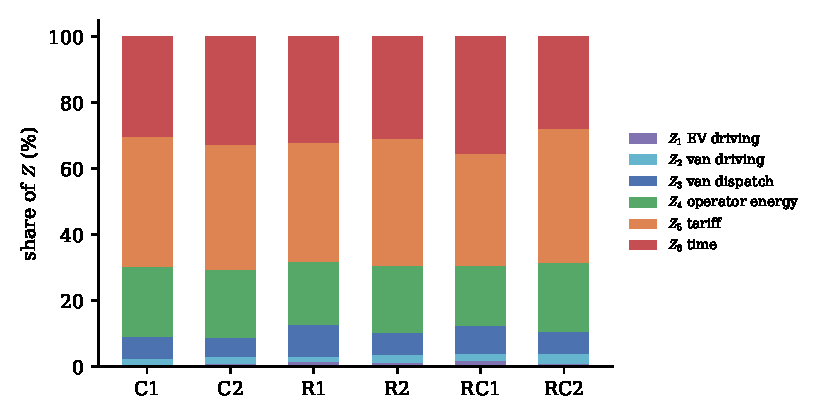
\includegraphics[width=0.6\textwidth]{figures/r_obj_family.pdf}
\caption{Composition of the objective by family (valid RL plans).}
\label{fig:objfamily}
\end{figure}

The short-horizon families R1 and RC1 have the fewest valid plans (\ValidRone{} of 120 and \ValidRCone{} of 80), as for the MILP. The composition of $Z$ is almost the same in every family: about 30\,\% operator cost and 70\,\% perceived customer cost, of which the perceived tariff is the largest part.

\inshort{Families differ in how often a plan exists and in cost level, not in cost structure.}

\subsection{EV-level distributions}
\begin{table}[H]\centering
\small
\caption{EV-level variables over all EVs of the valid RL plans (unless stated).}\label{tab:evstats}
\begin{adjustbox}{max width=\textwidth}\begin{tabular}{lrrrrrr}\toprule
variable (per EV) & count & mean & median & 10th pct & 90th pct & max \\ \midrule
income $\theta$ & 26\,050 & 0.46 & 0.42 & 0.18 & 0.82 & 1.00 \\
energy demand $E_i$ (kWh) & 26\,050 & 19.6 & 18.6 & 13.7 & 27.8 & 40.0 \\
nearest reachable FCS (km) & 22\,145 & 1.63 & 1.53 & 0.66 & 2.75 & 4.71 \\
demand pressure & 22\,145 & 0.53 & 0.24 & 0.03 & 1.59 & 2.66 \\
drive to FCS (km), FCS users & 21\,547 & 2.72 & 1.86 & 0.72 & 5.88 & 23.44 \\
FCS queue (min), FCS users & 21\,547 & 2.61 & 0.00 & 0.00 & 11.65 & 54.92 \\
van wait (min), van users & 4\,503 & 26.2 & 0.0 & 0.0 & 80.5 & 577.1 \\
charging time (min) & 26\,050 & 51.1 & 44.0 & 31.0 & 75.7 & 109.1 \\
request to charged (min) & 26\,050 & 66.4 & 61.4 & 42.3 & 98.1 & 608.1 \\
money paid (Rs) & 26\,050 & 335 & 326 & 232 & 510 & 1000 \\
perceived money (Rs) & 26\,050 & 349 & 320 & 192 & 530 & 1238 \\
perceived time (Rs) & 26\,050 & 278 & 217 & 118 & 515 & 1834 \\
perceived total (Rs) & 26\,050 & 628 & 583 & 408 & 916 & 2285 \\
\bottomrule\end{tabular}\end{adjustbox}\end{table}


\begin{figure}[H]
\centering
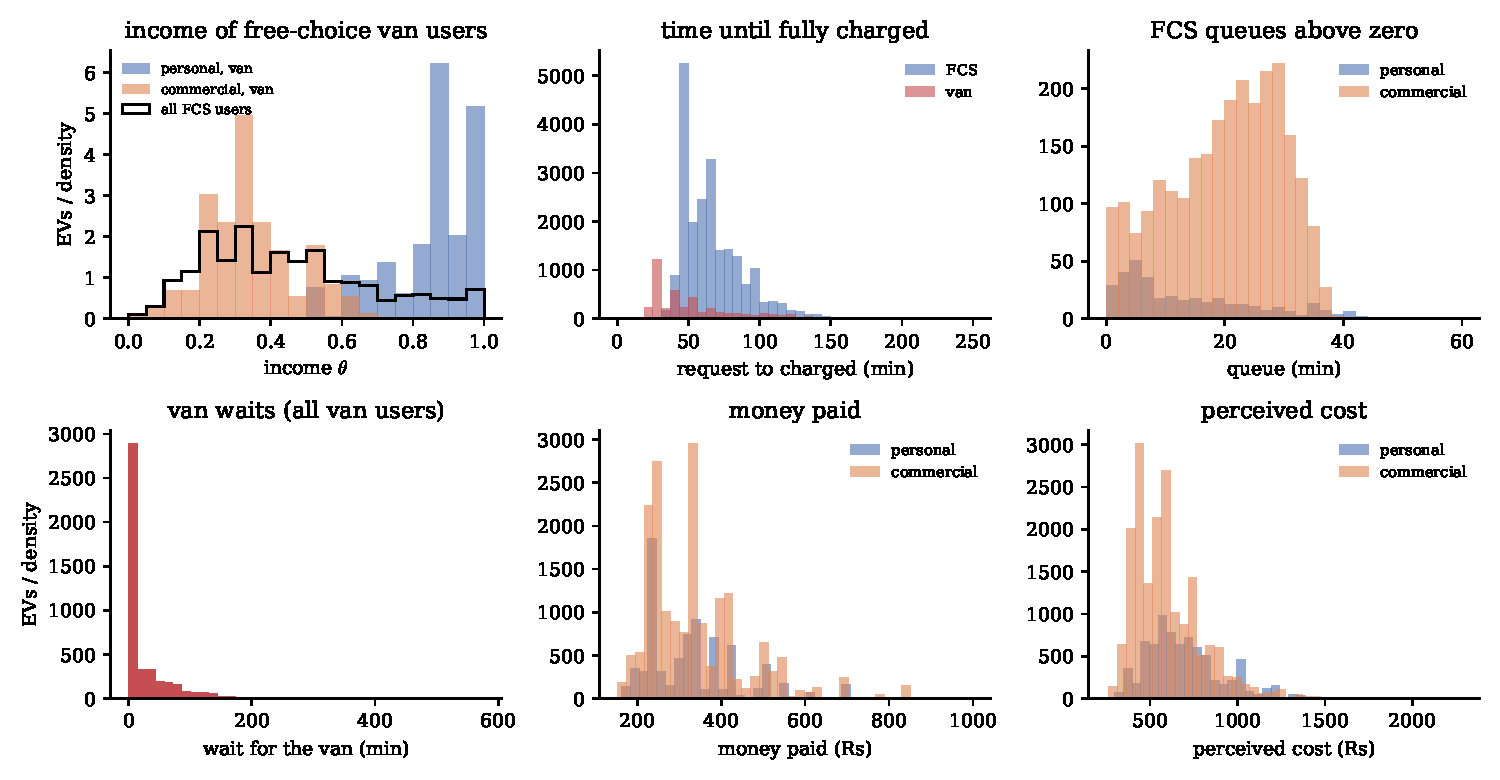
\includegraphics[width=0.95\textwidth]{figures/r_ev_dists.pdf}
\caption{Income of free-choice van users by segment, time until charged, queues, van waits, money paid and perceived cost (valid RL plans).}
\label{fig:evdists}
\end{figure}

\begin{itemize}
  \item Free-choice van users are mostly rich personal owners (top left). Commercial cars are \CommShareVanFree\pct{} of them, with a mean income of only \ThetaVanComm: they get a van because of queues, not income (Section~\ref{sec:pressure}).
  \item Most EVs are fully charged \ToChargedLo--\ToChargedHi{} minutes after their request (10th to 90th percentile).
  \item \QueueersFcs{} of the \FcsUsersFree{} free-choice station users queue at all; most of the queueing is done by commercial cars.
  \item \VanWaitZero\pct{} of van users do not wait for the van at all; the rest form a long tail.
\end{itemize}

\subsection{Correlations}
\begin{figure}[H]
\centering
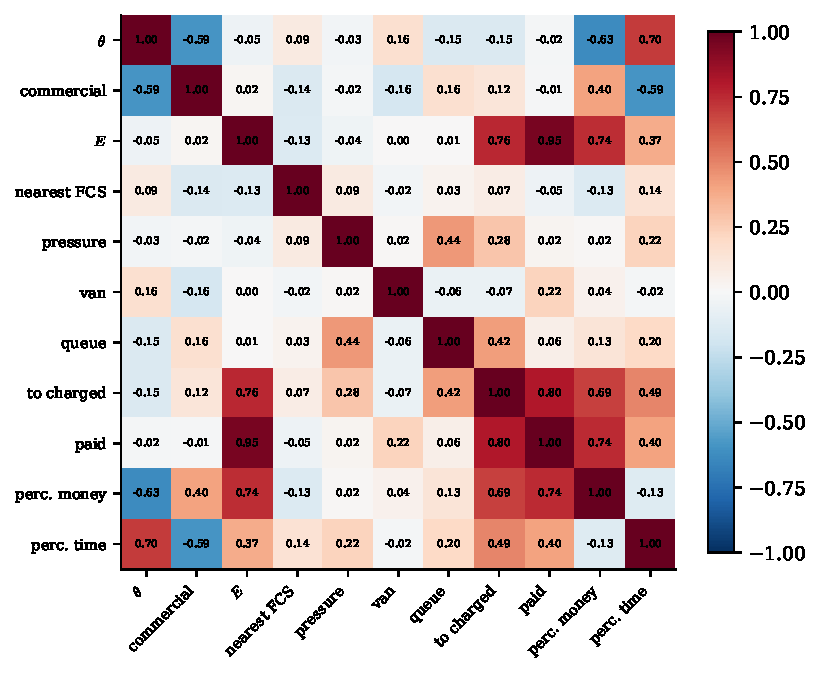
\includegraphics[width=0.45\textwidth]{figures/r_corr.pdf}
\caption{Spearman correlations between EV-level variables (free-choice EVs of valid RL plans).}
\label{fig:corr}
\end{figure}

Income goes with a van ($\rho=\RhoThetaVan$), being commercial against it ($\rho=\RhoSegVan$), and income with shorter queues ($\rho=\RhoThetaQueue$). Demand pressure is the strongest correlate of queueing ($\rho=\RhoPressQueue$), and energy of money paid ($\rho=\RhoEPaid$).

\inshort{Income and segment go with the van, pressure with queues, energy with money: the same pattern as the MILP, in weaker form for the van.}

%=====================================================================
\clearpage
\part{Comprehensive analysis}

\section{Analysis point by point}

\subsection{Solution quality against the MILP and the greedy rule}
\label{sec:quality}

\begin{figure}[H]
\centering
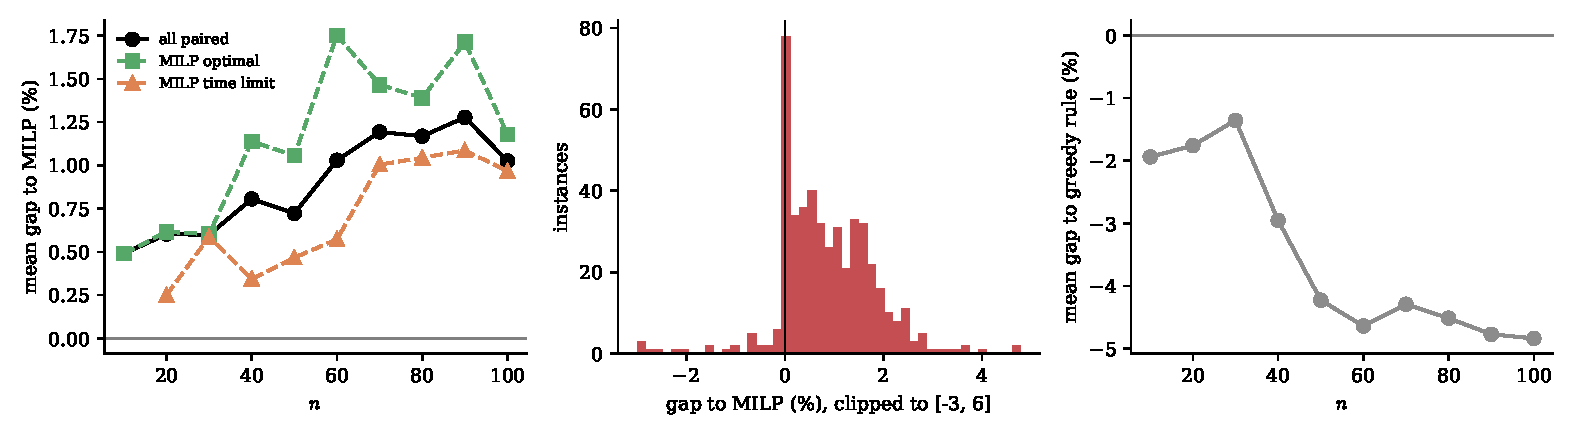
\includegraphics[width=\textwidth]{figures/r_gap.pdf}
\caption{Left: mean gap of RL to the MILP by size, overall and by MILP status. Middle: distribution of the gap. Right: mean gap of RL to the greedy rule.}
\label{fig:gap}
\end{figure}

\begin{table}[H]\centering
\small
\caption{Gap of RL to the MILP (\%) by instance size over instances where both are valid; vs optimal / vs time-limit = only MILP plans of that status; RL cheaper = negative gap; last column: gap to the greedy rule.}\label{tab:qualityn}
\begin{adjustbox}{max width=\textwidth}\begin{tabular}{lrrrrrrrr}\toprule
$n$ & paired & gap mean & gap median & vs optimal & vs time-limit & RL cheaper & equal ($\le$0.01\%) & vs greedy \\ \midrule
10 & 55 & 0.49 & 0.00 & 0.49 & -- & 0 & 38 & -1.94 \\
20 & 55 & 0.60 & 0.24 & 0.62 & 0.25 & 0 & 15 & -1.76 \\
30 & 55 & 0.60 & 0.30 & 0.60 & 0.59 & 0 & 1 & -1.36 \\
40 & 55 & 0.81 & 0.65 & 1.14 & 0.34 & 2 & 0 & -2.95 \\
50 & 53 & 0.72 & 0.69 & 1.06 & 0.47 & 5 & 0 & -4.23 \\
60 & 49 & 1.03 & 1.23 & 1.75 & 0.57 & 6 & 0 & -4.64 \\
70 & 44 & 1.19 & 1.28 & 1.47 & 1.00 & 3 & 0 & -4.29 \\
80 & 39 & 1.17 & 1.11 & 1.39 & 1.04 & 4 & 0 & -4.51 \\
90 & 36 & 1.28 & 1.38 & 1.71 & 1.09 & 4 & 0 & -4.77 \\
100 & 33 & 1.02 & 0.99 & 1.18 & 0.97 & 4 & 0 & -4.84 \\
\midrule all & 474 & 0.85 & 0.76 & 0.92 & 0.76 & 28 & 54 & -3.33 \\
\bottomrule\end{tabular}\end{adjustbox}\end{table}

\begin{table}[H]\centering
\small
\caption{Gap of RL to the MILP and to the greedy rule by family (\%).}\label{tab:qualityclass}
\begin{adjustbox}{max width=\textwidth}\begin{tabular}{lrrrrrrrr}\toprule
family & paired & gap mean & gap median & vs optimal & RL cheaper & paired greedy & vs greedy & beats greedy (\%) \\ \midrule
C1 & 89 & 0.84 & 0.84 & 0.86 & 3 & 89 & -1.97 & 79.8 \\
C2 & 79 & 1.66 & 1.80 & 1.79 & 4 & 79 & -0.85 & 50.6 \\
R1 & 75 & 0.38 & 0.31 & 0.26 & 6 & 74 & -2.79 & 83.8 \\
R2 & 110 & 1.16 & 1.26 & 1.12 & 4 & 110 & -3.42 & 77.3 \\
RC1 & 42 & 0.12 & 0.33 & 0.26 & 8 & 30 & -8.45 & 90.0 \\
RC2 & 79 & 0.48 & 0.46 & 0.17 & 3 & 79 & -5.75 & 86.1 \\
\bottomrule\end{tabular}\end{adjustbox}\end{table}


\begin{itemize}
  \item \textbf{Against the MILP.} Over the \NPaired{} paired instances RL costs \GapMean\pct{} more on average (median \GapMed\pct, 90th percentile \GapP\pct, worst \GapMax\pct).
  \item \textbf{Against proven optima.} The gap is \GapOpt\pct{} over the \NPairedOpt{} optimal MILP plans. RL equals the optimum within 0.01\,\% in \RLequalOpt{} of them and is never cheaper (\RLbelowOpt{} cases), as it must be.
  \item \textbf{Against time-limit plans.} The gap is \GapTl\pct, and RL is cheaper than the MILP in \RLbetterTl{} of them.
  \item \textbf{By size.} The gap grows with size, from \GapTen\pct{} at $n=10$ to \GapMaxNVal\pct{} at $n=\GapMaxN$. It is \GapHundred\pct{} at $n=100$, where the MILP itself often stops far from optimal.
  \item \textbf{By family.} RL is closest in \GapBestFam{} (\GapBestFamVal\pct), a short-horizon family where the MILP struggles. It is furthest in \GapWorstFam{} (\GapWorstFamVal\pct), with long horizons and clustered customers, where good orders are many and the MILP has time to find them.
  \item \textbf{Against the greedy rule.} RL beats the rule in \GreedyBeat{} of \GreedyN{} paired instances and is \GreedyGapAbs\pct{} cheaper on average. It is dearer in \GreedyWorse: the learned policy is a strict improvement on its teacher only on average.
\end{itemize}

\inshort{RL is within 1\,\% of the MILP on average and finds the optimum of many small instances. It costs most on large clustered instances with long horizons and least where the MILP struggles.}

\subsection{Feasibility: where RL fails}
\label{sec:feasibility}

\begin{table}[H]\centering
\caption{Rules broken by the invalid RL plans (a plan can break several).}\label{tab:violations}
\begin{adjustbox}{max width=\textwidth}\begin{tabular}{lrr}\toprule
violated rule & plans & violations \\ \midrule
EV finishes after $T$ & 39 & 60 \\
van back at the depot after $T$ & 38 & 45 \\
queue longer than $W_i$ & 13 & 13 \\
van battery exceeded & 1 & 1 \\
\bottomrule\end{tabular}\end{adjustbox}\end{table}

\begin{table}[H]\centering
\caption{Invalid RL plans by family. Last column: instances where an EV the policy could not place cannot be fully charged by $T$ even alone (free gun at once, or a van leaving for it at once).}\label{tab:invalid}
\begin{adjustbox}{max width=\textwidth}\begin{tabular}{lrrrrrrr}\toprule
family & invalid & smallest $n$ & largest $n$ & MILP infeasible & MILP no plan & unplaced EVs (mean) & one EV alone impossible \\ \midrule
C2 & 1 & 100 & 100 & 0 & 1 & 1.0 & 0 \\
R1 & 31 & 50 & 100 & 29 & 2 & 2.1 & 29 \\
RC1 & 28 & 10 & 100 & 22 & 6 & 1.9 & 20 \\
\bottomrule\end{tabular}\end{adjustbox}\end{table}


\begin{itemize}
  \item \textbf{RL never fails where a plan is known.} All \NInvalid{} invalid RL plans are on instances without a MILP plan: \InvalidInf{} proven infeasible and \InvalidNoPlan{} unsolved.
  \item \textbf{Mostly the data.} In \InvLone{} of the \InvalidInf{} infeasible instances, a car the policy could not place cannot be fully charged by $T$ even alone, with a free gun at once or a van leaving for it at once. Almost all are in R1 (\InvFamR) and RC1 (\InvFamRC), where $T$ is only 230--240 minutes. In \InvOneEV{} plans only one car is unplaced; the most is \InvDroppedMax.
  \item \textbf{Which rules break.} After appending the unplaced cars, a plan typically has a car finishing after $T$ (\InvAfterT{} plans) or a van back after $T$ (\InvVanBack{} plans). Queues longer than the patience $W_i$ appear in \InvQueue{} plans, mainly in the \InvalidNoPlan{} large, congested instances that the MILP could not solve either.
  \item \textbf{Open cases.} For those \InvalidNoPlan{} instances none of the unplaced cars is impossible alone. It is not known whether a plan exists: neither method found one.
  \item \textbf{Where RL helps.} RL finds plans for \RLonly{} instances without a MILP plan (\RLonlyFams; mean size $n=\RLonlyMeanN$), and for \RLonlyGr{} without a greedy plan. These are the large, congested instances where Gurobi's search ran out of time.
\end{itemize}

\inshort{RL's failures are infeasible data or open instances that no method has solved; where a plan is known, RL finds one too. Its value is greatest on the large congested instances.}

\subsection{Computation and the value of learning}
\label{sec:compute}

\begin{figure}[H]
\centering
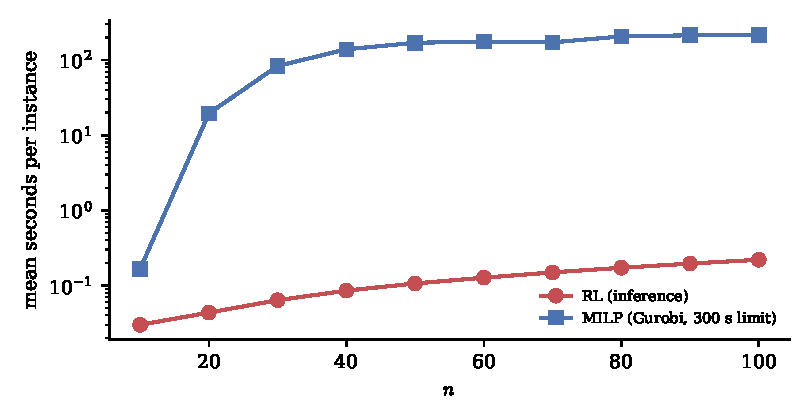
\includegraphics[width=0.6\textwidth]{figures/r_time.pdf}
\caption{Mean time per instance by size (log scale).}
\label{fig:time}
\end{figure}

\begin{itemize}
  \item RL needs \RLtime\,s per instance on average (\RLtimeHundred\,s at $n=100$), the MILP \MILPtime\,s (\MILPtimeHundred\,s at $n=100$): about \Speedup{} times faster.
  \item All \NInst{} instances take \RLtotalS\,s with RL against \MILPtotalH{} CPU-hours of MILP solving.
  \item Training took \TrainMinBest{} minutes up to the best model. It pays for itself after about \BreakEven{} instances. In the experiments the same model is reused without retraining (results report).
\end{itemize}

\inshort{Inference costs a tenth of a second; after a short training the method is three orders of magnitude faster than the MILP.}

\subsection{Anatomy of the objective: where RL loses}
\label{sec:anatomy}

\begin{table}[H]\centering
\caption{Composition of $Z$ over the paired instances and where the RL's extra cost comes from.}\label{tab:terms}
\begin{adjustbox}{max width=\textwidth}\begin{tabular}{lrrr}\toprule
term & RL share of $Z$ (\%) & MILP share (\%) & RL $-$ MILP (\% of MILP $Z$) \\ \midrule
$Z_1$ EV driving & 1.0 & 0.9 & 0.12 \\
$Z_2$ van driving & 2.3 & 2.4 & -0.08 \\
$Z_3$ van dispatch & 7.0 & 7.5 & -0.40 \\
$Z_4$ operator energy & 20.5 & 20.9 & -0.23 \\
$Z_5$ tariff (perceived) & 38.5 & 39.3 & -0.44 \\
$Z_6$ time (perceived) & 30.7 & 29.0 & 2.00 \\
total $Z$ & 100.0 & 100.0 & 0.97 \\
\bottomrule\end{tabular}\end{adjustbox}\end{table}


\begin{figure}[H]
\centering
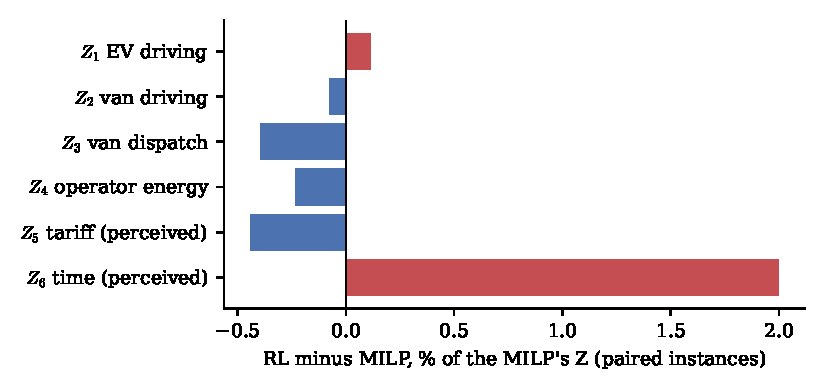
\includegraphics[width=0.62\textwidth]{figures/r_terms.pdf}
\caption{Difference of each term of $Z$, RL minus MILP, as a share of the MILP's $Z$ (paired instances).}
\label{fig:terms}
\end{figure}

RL's extra cost is customer time ($Z_6$: +\TermDSix{} points of $Z$), above all the longer queues at stations. It is partly offset by lower perceived tariff ($Z_5$: \TermDFive), van dispatch ($Z_3$: \TermDThree) and operator energy ($Z_4$: \TermDFour). All three come from serving fewer customers by van: van energy and the van tariff are dearer than the station's. The structure is otherwise the same: operator cost \OpShareRL\pct, perceived tariff \TariffShareRL\pct{} and perceived time \TimeShareRL\pct{} of $Z$.

\subsubsection{Elasticities (envelope theorem)}
As in the MILP report, every term of $Z$ is a coefficient times a quantity of the plan, and $\partial Z/\partial c_k$ is that quantity for a fixed plan. The elasticity of $Z$ with respect to $c_k$ is then the share of $Z$ carried by $c_k$. The elasticities add up to \ElSumRL\pct{} rather than 100\,\%, because the money terms $Z_1$ and $Z_5$ (\MoneyShareRL\pct{} of $Z$) are products $\mu\times$price and are counted for both factors.

\begin{table}[H]\centering
\small
\caption{Elasticity of $Z$ (share of $Z$ carried by each coefficient, envelope theorem) in the RL plans and the MILP plans of the paired instances. Superscripts: activity, segment (P personal, C commercial), end point ($\theta=0$ or 1).}\label{tab:elasticity}
\begin{adjustbox}{max width=\textwidth}\begin{tabular}{lrrrr}\toprule
coefficient & value & elasticity RL (\%) & elasticity MILP (\%) & difference \\ \midrule
$p^{\mathrm F}$ & 15 & 29.26 & 28.88 & 0.38 \\
$\mu^{\mathrm{C,0}}$ & 1.5 & 25.68 & 25.87 & -0.19 \\
$\pi^{\mathrm F}$ & 8.7 & 16.14 & 15.66 & 0.48 \\
$c^{\mathrm{C,P,1}}$ & 10 & 9.92 & 8.23 & 1.70 \\
$p^{\mathrm M}$ & 25 & 9.27 & 10.46 & -1.19 \\
$c^{\mathrm{C,C,1}}$ & 6 & 7.65 & 7.75 & -0.09 \\
$c^{\mathrm F}_m$ & 1500 & 7.02 & 7.48 & -0.46 \\
$\mu^{\mathrm{P,0}}$ & 1.5 & 5.16 & 5.31 & -0.15 \\
$\mu^{\mathrm{C,1}}$ & 0.5 & 4.84 & 4.87 & -0.02 \\
$\pi^{\mathrm M}$ & 10.7 & 4.35 & 5.26 & -0.90 \\
$\mu^{\mathrm{P,1}}$ & 0.5 & 3.82 & 4.17 & -0.35 \\
$c^{\mathrm{C,C,0}}$ & 1.5 & 3.49 & 3.52 & -0.03 \\
$c^{\mathrm M}$ & 15 & 2.33 & 2.42 & -0.10 \\
$c^{\mathrm{D,P,1}}$ & 15 & 2.19 & 1.72 & 0.47 \\
$c^{\mathrm{V,C,1}}$ & 6 & 1.87 & 1.79 & 0.08 \\
$c^{\mathrm{D,C,1}}$ & 6 & 1.44 & 1.26 & 0.18 \\
$c^{\mathrm{V,P,1}}$ & 5 & 1.25 & 2.19 & -0.94 \\
$c^{\mathrm{EV}}$ & 4 & 0.99 & 0.88 & 0.11 \\
$c^{\mathrm{V,C,0}}$ & 1.5 & 0.80 & 0.80 & -0.00 \\
$c^{\mathrm{D,C,0}}$ & 1.5 & 0.65 & 0.58 & 0.07 \\
$c^{\mathrm{C,P,0}}$ & 1 & 0.46 & 0.45 & 0.01 \\
$c^{\mathrm{Q,C,1}}$ & 7.5 & 0.39 & 0.23 & 0.15 \\
$c^{\mathrm{Q,C,0}}$ & 2 & 0.23 & 0.15 & 0.08 \\
$c^{\mathrm{Q,P,1}}$ & 25 & 0.13 & 0.10 & 0.04 \\
$c^{\mathrm{D,P,0}}$ & 1.5 & 0.11 & 0.10 & 0.00 \\
$c^{\mathrm{V,P,0}}$ & 0.5 & 0.05 & 0.07 & -0.02 \\
$c^{\mathrm{Q,P,0}}$ & 2.5 & 0.01 & 0.01 & -0.00 \\
\bottomrule\end{tabular}\end{adjustbox}\end{table}


\begin{figure}[H]
\centering
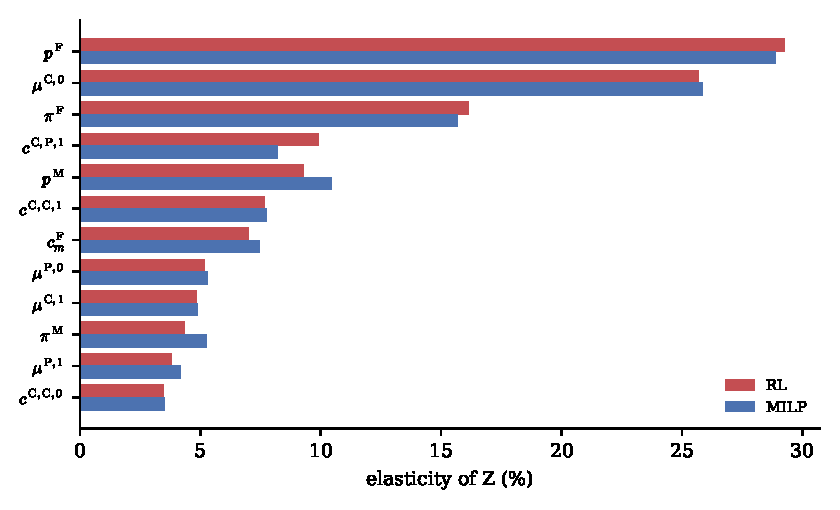
\includegraphics[width=0.6\textwidth]{figures/r_elasticity.pdf}
\caption{Elasticity of $Z$ for the twelve most influential coefficients, RL against MILP.}
\label{fig:elasticity}
\end{figure}

\begin{itemize}
  \item The most influential coefficients are the same for RL and MILP: the station tariff \ElTopOne{} (\ElTopOneV\pct), the money sensitivity of the poorest commercial drivers \ElTopTwo{} (\ElTopTwoV\pct), the grid price \ElTopThree{} (\ElTopThreeV\pct) and the value of station-charging time of rich personal owners \ElTopFour{} (\ElTopFourV\pct).
  \item The largest difference is \ElDiffCoef{} (RL \ElDiffRL\pct, MILP \ElDiffM\pct): RL keeps more rich personal owners at stations, so their charging minutes weigh more.
  \item The commercial segment carries most of the money terms because 70\,\% of the cars are commercial and their incomes are low.
\end{itemize}

\inshort{RL loses on customer time and gains a little on tariff, energy and dispatch: the signature of a plan with fewer vans. The cost structure and the elasticities are nearly identical to the MILP's.}

\subsection{Decision agreement with the MILP}
\label{sec:agreement}

\begin{table}[H]\centering
\small
\caption{Decisions of RL and MILP for the same free-choice EV (paired instances). Same station: share of EVs both send to a station that go to the same station.}\label{tab:confusion}
\begin{adjustbox}{max width=\textwidth}\begin{tabular}{lrrrrrrr}\toprule
segment & EVs & both FCS & RL FCS, MILP van & RL van, MILP FCS & both van & same type (\%) & same station (\%) \\ \midrule
personal & 6\,095 & 4\,743 & 959 & 138 & 255 & 82.0 & 89.0 \\
commercial & 14\,125 & 13\,948 & 78 & 74 & 25 & 98.9 & 75.5 \\
all & 20\,220 & 18\,691 & 1\,037 & 212 & 280 & 93.8 & 78.9 \\
\bottomrule\end{tabular}\end{adjustbox}\end{table}


RL makes the same station-or-van choice as the MILP for \AgreeType\pct{} of free-choice EVs (\AgreePers\pct{} of personal ones), and of those both send to a station, \AgreeStation\pct{} go to the same station. The disagreements are one-sided: \MilpVanRlFcs{} EVs get a van from the MILP but a station from RL, against \RlVanMilpFcs{} the other way. The personal EVs the MILP sends by van are rich (mean $\theta=\MilpVanPersThetaMean$); RL keeps only \MilpVanPersKeptRl\pct{} of them on a van.

\inshort{RL agrees with the MILP on most decisions; where it differs, it is almost always by sending a rich personal owner to a station instead of a van.}

\subsection{Segment, income and the choice of resource}
\label{sec:income}

\textbf{Theory.} For a typical EV (20\,kWh, 2\,km to its station, no queue, 10-minute van wait, 4\,km van detour), formulation 4 gives the extra cost of a van $\Delta(\theta)$:
\begin{itemize}
  \item \textbf{Personal:} \DeltaZeroP{} Rs at $\theta=0$ and \DeltaOneP{} Rs at $\theta=1$, so the van wins above $\theta^{*}=\ThetaStarP$ (the threshold of formulation 3).
  \item \textbf{Commercial:} \DeltaZeroC{} and \DeltaOneC{} Rs, positive at every income, so a taxi does not take a van off-peak.
  \item \textbf{A van sent for this EV alone:} if the dispatch cost must be paid for it, even the richest personal owner has $\Delta(1)=\DeltaOnePDispatch$ Rs. Vans leave for stranded EVs, and free-choice customers fill the spare seats.
\end{itemize}

\begin{figure}[H]
\centering
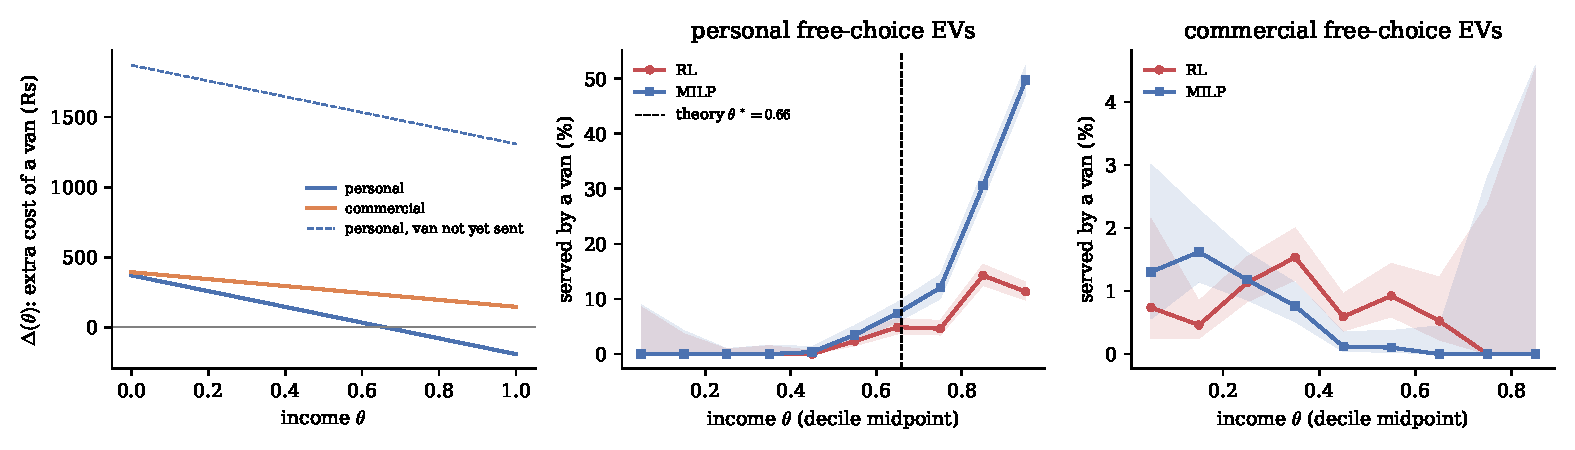
\includegraphics[width=\textwidth]{figures/r_van_income.pdf}
\caption{Left: theory, extra cost of a van $\Delta(\theta)$ for the typical EV by segment (dashed: van not yet sent). Middle and right: share of free-choice EVs served by a van by income decile and segment, RL against MILP (95\,\% Wilson band).}
\label{fig:vanincome}
\end{figure}

\begin{table}[H]\centering
\small
\caption{Van share of free-choice EVs by segment and income band; 95\,\% Wilson interval for RL; all valid plans of each method.}\label{tab:vanband}
\begin{adjustbox}{max width=\textwidth}\begin{tabular}{llrrrrr}\toprule
segment & income $\theta$ & EVs (RL) & by van RL (\%) & 95\% interval & EVs (MILP) & by van MILP (\%) \\ \midrule
personal & 0.0--0.2 & 141 & 0.0 & [0.0, 2.7] & 125 & 0.0 \\
 & 0.2--0.4 & 652 & 0.0 & [0.0, 0.6] & 608 & 0.0 \\
 & 0.4--0.6 & 1\,322 & 1.4 & [0.9, 2.1] & 1\,181 & 2.1 \\
 & 0.6--0.8 & 1\,896 & 4.7 & [3.9, 5.8] & 1\,668 & 9.8 \\
 & 0.8--1.0 & 2\,716 & 12.7 & [11.5, 14.0] & 2\,513 & 40.8 \\
commercial & 0.0--0.2 & 2\,572 & 0.5 & [0.3, 0.9] & 2\,297 & 1.6 \\
 & 0.2--0.4 & 6\,901 & 1.3 & [1.1, 1.6] & 6\,363 & 1.0 \\
 & 0.4--0.6 & 4\,754 & 0.7 & [0.5, 1.0] & 4\,398 & 0.1 \\
 & 0.6--0.8 & 1\,110 & 0.5 & [0.2, 1.1] & 987 & 0.0 \\
 & 0.8--1.0 & 81 & 0.0 & [0.0, 4.5] & 80 & 0.0 \\
\bottomrule\end{tabular}\end{adjustbox}\end{table}


\begin{itemize}
  \item \textbf{The segment pattern holds.} In RL plans \VanRPers\pct{} of free-choice personal cars get a van, against \VanRComm\pct{} of commercial cars (MILP: \VanMPers\pct{} and \VanMComm\pct).
  \item \textbf{The income step holds, but comes later and lower.} RL's personal van share exceeds 5\,\% only at $\theta$ \StepR{} (MILP \StepM; theory $\theta^{*}=\ThetaStarP$) and reaches \VanTopRPers\pct{} in the richest band, against \VanTopMPers\pct{} for the MILP. Below $\theta=0.4$ RL gives personal owners no vans (\VanLowRPers\pct).
  \item \textbf{Van users are richer than station users:} mean $\theta$ \ThetaVanR{} against \ThetaFcsR{} among personal cars.
  \item \textbf{Commercial cars get vans only at high pressure} (Section~\ref{sec:pressure}), as the theory predicts.
\end{itemize}

\begin{table}[H]\centering
\small
\caption{Logistic regression of $P$(served by a van) over the 22\,145 free-choice EVs of the valid RL plans.}\label{tab:logit}
\begin{adjustbox}{max width=\textwidth}\begin{tabular}{lrrrr}\toprule
term & coefficient & std. error & $z$ & $p$-value \\ \midrule
intercept & -7.422 & 0.391 & -19.0 & $<0.001$ \\
income $\theta$ & 6.711 & 0.377 & 17.8 & $<0.001$ \\
commercial & 0.744 & 0.356 & 2.1 & 0.037 \\
$\theta\times$ commercial & -3.244 & 0.644 & -5.0 & $<0.001$ \\
high pressure & 4.211 & 0.316 & 13.3 & $<0.001$ \\
$\theta\times$ high pressure & -5.102 & 0.420 & -12.1 & $<0.001$ \\
energy $E_i$ (per 10 kWh) & 0.028 & 0.074 & 0.4 & 0.709 \\
nearest reachable FCS (km) & -0.390 & 0.059 & -6.6 & $<0.001$ \\
\bottomrule\end{tabular}\end{adjustbox}\end{table}


The logistic regression confirms the pattern. An increase of $\theta$ by 0.1 raises a personal car's probability of a van by \AmePers{} percentage points on average; for a commercial car the effect is nil (\AmeComm{} points). The AUC is \LogitAUC. Because only a few per cent get a van, the classification accuracy (\LogitAcc\pct) equals the share of station users (\LogitBaseRate\pct) and is not informative.

\inshort{RL reproduces the theory's direction: vans for rich personal owners, stations for taxis. But its step is later and much lower than the MILP's; it under-uses the driver-free benefit of rich private owners.}

\subsection{Shadow prices of RL plans}
\label{sec:duals}

The method is that of the MILP report: fix every yes/no decision of a plan and re-solve the timing LP in the start times and waits. Its duals are the shadow prices of the plan. For all \LPPlansR{} RL plans and \LPPlansM{} MILP plans the LP optimum equals the plan's own waiting cost to the last digit: RL's earliest-start timing is optimal for its decisions.

\begin{table}[H]\centering
\footnotesize
\caption{Shadow prices of the fixed-plan LPs (absolute values, Rs/min) of every valid RL and MILP plan.}\label{tab:duals}
\begin{adjustbox}{max width=\textwidth}\begin{tabular}{lrrrrrrp{3.2cm}}\toprule
constraint & rows RL & non-zero (\%) & mean if $\neq0$ & rows MILP & non-zero (\%) & mean if $\neq0$ & meaning \\ \midrule
FCS arrival $S_i\ge r_i+t_{if}$ & 21\,547 & 11.0 & 6.70 & 18\,903 & 7.6 & 5.00 & not unique (degenerate); not interpreted \\
van release $S_i\ge r_i$ & 4\,503 & 51.2 & 3.99 & 4\,927 & 54.0 & 4.26 & not unique (degenerate); not interpreted \\
gun order $S_j\ge S_i+\tau^{\mathrm F}_i$ & 12\,454 & 23.4 & 6.75 & 10\,829 & 13.5 & 5.14 & value of one gun-minute \\
van order $S_j\ge S_i+\tau^{\mathrm M}_i+t_{ij}$ & 3\,398 & 41.5 & 5.47 & 3\,887 & 38.7 & 5.51 & value of one van-minute \\
first stop $S_a\ge t_{0a}$ & 1\,105 & 70.1 & 7.84 & 1\,040 & 72.6 & 8.31 & value of an earlier van departure \\
queue limit $q^{\mathrm F}_i\le W_i$ & 21\,547 & 0.0 & 0.00 & 18\,903 & 0.0 & 0.00 & one more minute of patience \\
deadline $C_i\le T$, van return & 27\,155 & 0.0 & 0.00 & 24\,870 & 0.0 & 0.00 & one more minute of horizon \\
\bottomrule\end{tabular}\end{adjustbox}\end{table}


\begin{figure}[H]
\centering
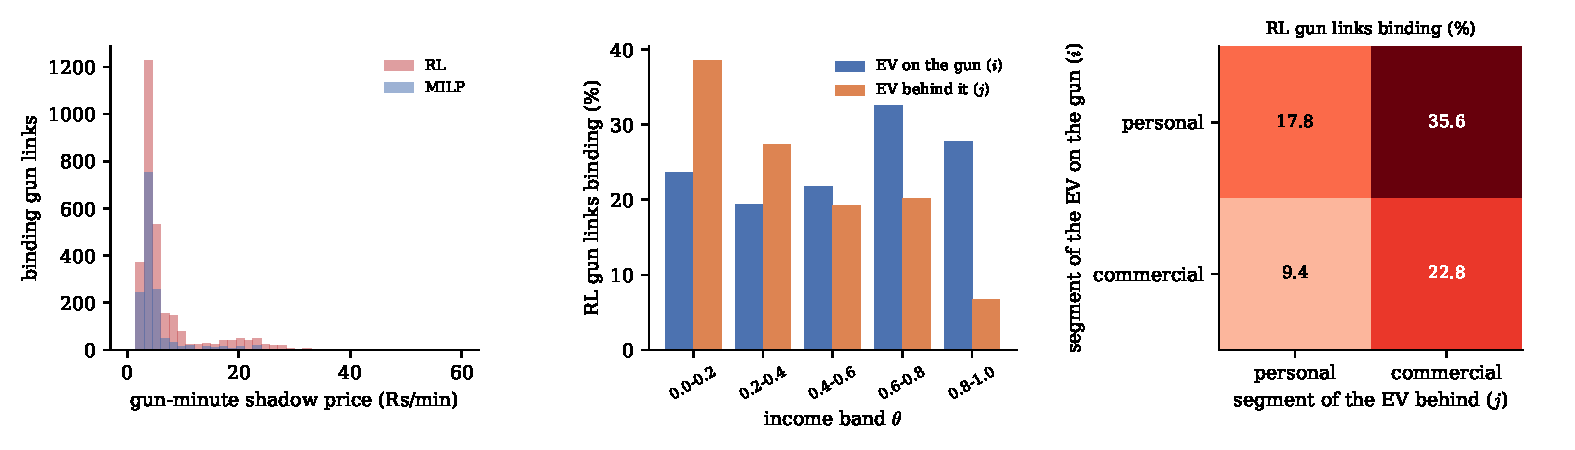
\includegraphics[width=\textwidth]{figures/r_gun_duals.pdf}
\caption{Left: gun-minute shadow prices where binding, RL and MILP. Middle: share of binding RL gun links by income of the EV on the gun and of the EV behind it. Right: share binding by segment of both.}
\label{fig:gunduals}
\end{figure}

\begin{table}[H]\centering
\small
\caption{Gun links (EV $i$ then EV $j$ on one gun) by the demand-pressure tercile of the EV behind (shared cut points, Section~\ref{sec:defs}).}\label{tab:gunpressure}
\begin{adjustbox}{max width=\textwidth}\begin{tabular}{llrrrr}\toprule
method & pressure of the EV behind & gun links & binding (\%) & mean dual if binding & mean dual, all links \\ \midrule
RL & low & 6\,554 & 2.0 & 5.3 & 0.11 \\
 & medium & 3\,191 & 14.7 & 6.6 & 0.97 \\
 & high & 2\,709 & 85.6 & 6.9 & 5.88 \\
MILP & low & 6\,437 & 0.7 & 4.1 & 0.03 \\
 & medium & 2\,840 & 6.6 & 5.3 & 0.35 \\
 & high & 1\,552 & 78.8 & 5.2 & 4.06 \\
\bottomrule\end{tabular}\end{adjustbox}\end{table}


\begin{itemize}
  \item \textbf{Gun-minutes are scarce more often.} \GunBindR\pct{} of the \GunLinksR{} consecutive gun links in RL plans are binding (MILP \GunBindM\pct). Where binding, a gun-minute is worth \GunPriceR{} Rs on average (MILP \GunPriceM).
  \item \textbf{Congestion is a peak phenomenon.} \GunBindHighR\pct{} of links are binding when the EV behind arrives at high pressure, against \GunBindLowR\pct{} at low pressure.
  \item \textbf{Who waits behind whom.} The EV waiting behind a binding link is poor more often (\BindPoorBehind\pct{} of links binding when the follower is in the poorest band, \BindRichBehind\pct{} in the richest). A commercial car waiting behind a personal one is the most frequent binding pair (\BindPC\pct).
  \item \textbf{Van-minutes} are binding on \VanBindR\pct{} of van legs (MILP \VanBindM\pct), worth \VanPriceR{} Rs/min when binding.
  \item \textbf{Zero shadow prices.} Patience limits and the deadline have zero shadow price in every plan of both methods. They act only by excluding plans.
\end{itemize}

\begin{figure}[H]
\centering
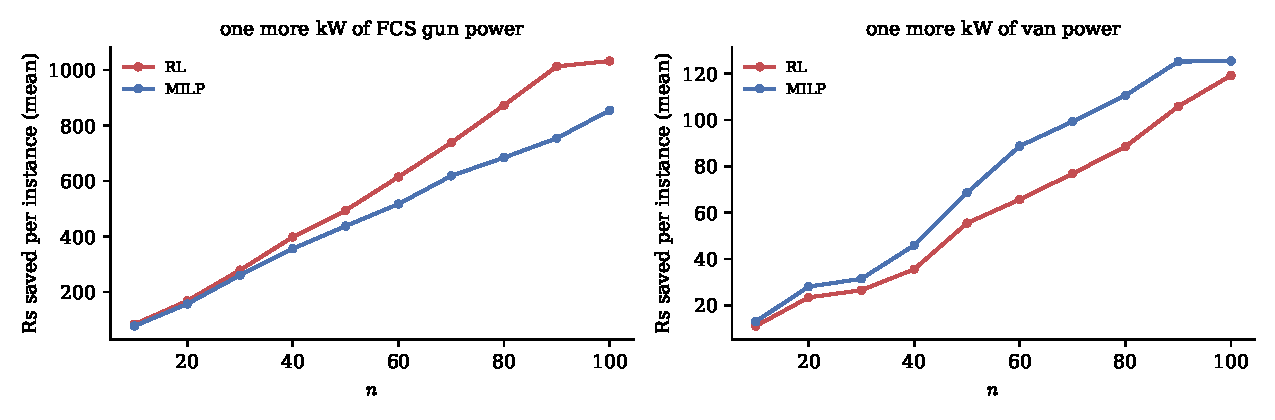
\includegraphics[width=0.8\textwidth]{figures/r_power.pdf}
\caption{Value of one more kW of charging power per instance (fixed decisions), by instance size.}
\label{fig:power}
\end{figure}

One more kW at every station gun is worth \PowerFR{} Rs per instance in RL plans (median \PowerFMedR), against \PowerFM{} Rs in MILP plans. \PowerCongR\pct{} of it is congestion relief (MILP \PowerCongM\pct). One more kW of van power is worth \PowerMR{} Rs (MILP \PowerMM).

\inshort{RL plans lean harder on the stations: gun-minutes are binding almost twice as often, faster guns are worth more, and the price of congestion is paid mostly by poorer and commercial customers waiting behind others.}

\subsection{Queues, priority and driving}
\label{sec:queues}

\begin{figure}[H]
\centering
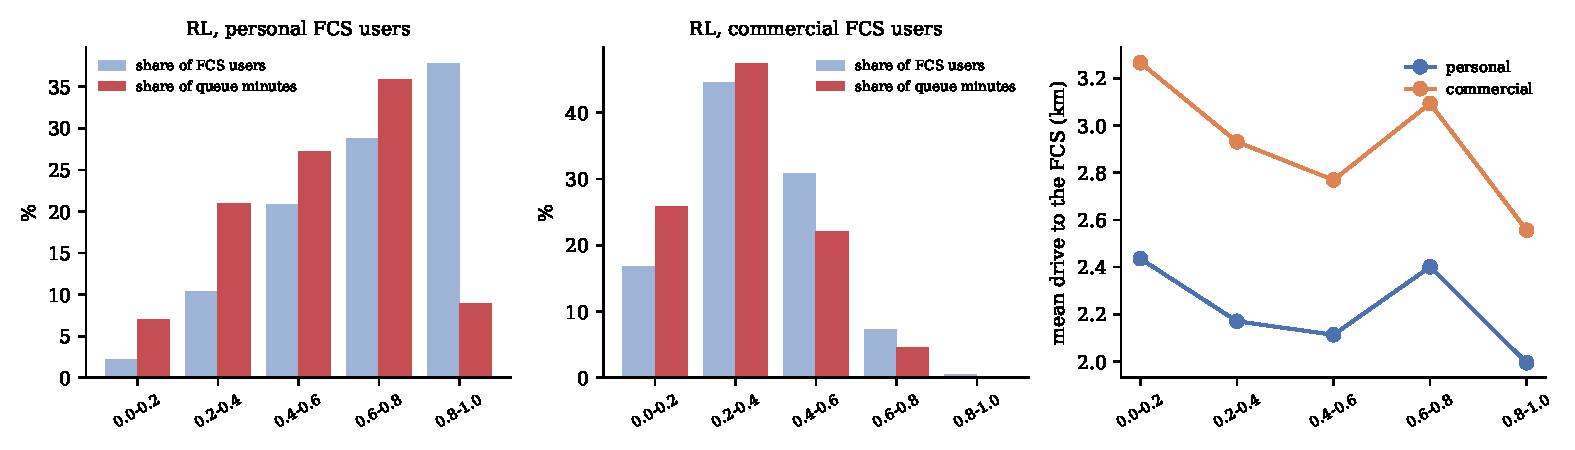
\includegraphics[width=\textwidth]{figures/r_queues.pdf}
\caption{Left and middle: share of station users and of queue minutes by income band, per segment. Right: mean distance driven to the station.}
\label{fig:queues}
\end{figure}

\begin{table}[H]\centering
\footnotesize
\caption{Station users of the RL plans by segment and income band (queues in minutes; shares within the segment).}\label{tab:queues}
\begin{adjustbox}{max width=\textwidth}\begin{tabular}{llrrrrrrrr}\toprule
segment & income $\theta$ & FCS users & users (\%) & queue min. (\%) & queueing (\%) & mean queue & longest & MILP mean queue & drive (km) \\ \midrule
personal & 0.0--0.2 & 141 & 2.2 & 7.1 & 10.6 & 2.47 & 54.9 & 1.45 & 2.44 \\
 & 0.2--0.4 & 652 & 10.4 & 20.9 & 4.9 & 1.58 & 42.2 & 1.32 & 2.17 \\
 & 0.4--0.6 & 1\,304 & 20.8 & 27.2 & 5.7 & 1.03 & 40.4 & 0.57 & 2.11 \\
 & 0.6--0.8 & 1\,806 & 28.8 & 35.8 & 8.7 & 0.98 & 30.1 & 0.18 & 2.40 \\
 & 0.8--1.0 & 2\,371 & 37.8 & 8.9 & 3.2 & 0.19 & 18.1 & 0.06 & 1.99 \\
commercial & 0.0--0.2 & 2\,559 & 16.8 & 25.8 & 22.6 & 5.18 & 38.5 & 2.77 & 3.27 \\
 & 0.2--0.4 & 6\,809 & 44.6 & 47.4 & 17.1 & 3.57 & 34.4 & 1.76 & 2.93 \\
 & 0.4--0.6 & 4\,719 & 30.9 & 22.1 & 13.9 & 2.40 & 29.7 & 0.92 & 2.77 \\
 & 0.6--0.8 & 1\,105 & 7.2 & 4.5 & 14.8 & 2.11 & 24.4 & 0.75 & 3.09 \\
 & 0.8--1.0 & 81 & 0.5 & 0.2 & 6.2 & 1.01 & 19.5 & 0.00 & 2.56 \\
\bottomrule\end{tabular}\end{adjustbox}\end{table}


\begin{itemize}
  \item \textbf{More queueing than the MILP.} \QueueersR\pct{} of RL station users queue (MILP \QueueersM\pct). Mean queues are \QueueRComm{} min for commercial and \QueueRPers{} min for personal users, against \QueueMComm{} and \QueueMPers{} in the MILP.
  \item \textbf{Commercial cars do the queueing:} \CommQShare\pct{} of all queue minutes for \CommUShare\pct{} of the station users.
  \item \textbf{Within a segment, the poor queue:} the two lowest commercial bands are \PoorUShareComm\pct{} of commercial station users but do \PoorQShareComm\pct{} of commercial queueing.
  \item \textbf{No patience limit is reached} (\PatienceHitR{} station users at $W_i$): queues follow from the cost weights alone.
\end{itemize}

\inshort{The cars that do not get a van queue: in RL plans more of them, mostly low-income commercial drivers, whose time is cheapest in the objective.}

\subsection{Peak and off-peak: demand pressure}
\label{sec:pressure}

Demand pressure and its terciles are defined in Section~\ref{sec:defs}. They depend only on the data, so they are the same for RL and MILP and in every report. \PressHighShareRL\pct{} of the free-choice EVs of the valid RL plans are in the high tercile; the policy never sees this measure and reacts only to the queues it builds.

\begin{figure}[H]
\centering
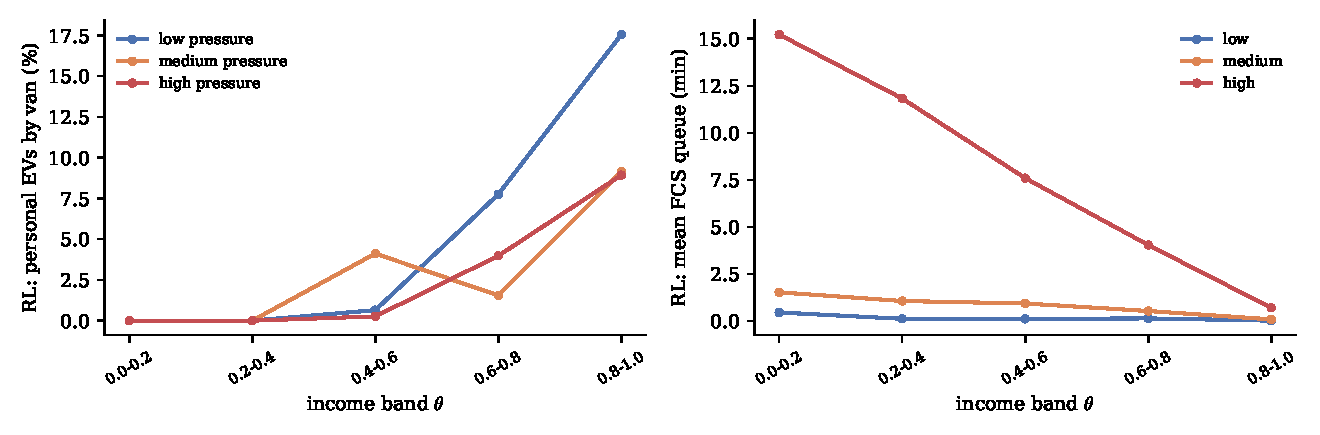
\includegraphics[width=0.9\textwidth]{figures/r_pressure.pdf}
\caption{RL: van share of personal free-choice EVs and mean station queue by income band, for low, medium and high demand pressure.}
\label{fig:pressure}
\end{figure}

\begin{table}[H]\centering
\small
\caption{Free-choice EVs of the valid plans by demand-pressure tercile (shared cut points), RL against MILP.}\label{tab:pressure}
\begin{adjustbox}{max width=\textwidth}\begin{tabular}{llrrrrr}\toprule
pressure & method & free-choice EVs & queueing (\%) & mean queue (min) & personal by van (\%) & commercial by van (\%) \\ \midrule
low & RL & 9\,602 & 1.4 & 0.14 & 9.4 & 0.0 \\
 & MILP & 9\,480 & 0.5 & 0.03 & 23.4 & 0.0 \\
medium & RL & 6\,748 & 7.1 & 0.90 & 5.1 & 0.0 \\
 & MILP & 6\,378 & 3.1 & 0.26 & 17.1 & 0.0 \\
high & RL & 5\,795 & 41.7 & 8.78 & 4.4 & 3.6 \\
 & MILP & 4\,362 & 30.3 & 5.52 & 16.6 & 3.4 \\
\bottomrule\end{tabular}\end{adjustbox}\end{table}


\begin{itemize}
  \item \textbf{Queues are a peak phenomenon:} mean queue \QueueRPressLow, \QueueRPressMedium{} and \QueueRPressHigh{} minutes at low, medium and high pressure.
  \item \textbf{At the peak, commercial cars start to get vans} (\VanCommPressHigh\pct{} at high pressure, \VanCommPressLow\pct{} at low). This is the theory's ``queues, not income, push taxis to vans''.
  \item \textbf{Fewer vans for personal cars at the peak:} \VanPersPressHigh\pct{} at high against \VanPersPressLow\pct{} at low pressure. The seats are then taken.
\end{itemize}

\inshort{Peak demand creates the queues and is the only time commercial cars win van seats, as formulation 4 predicts.}

\subsection{Planning horizon and layout}

\begin{figure}[H]
\centering
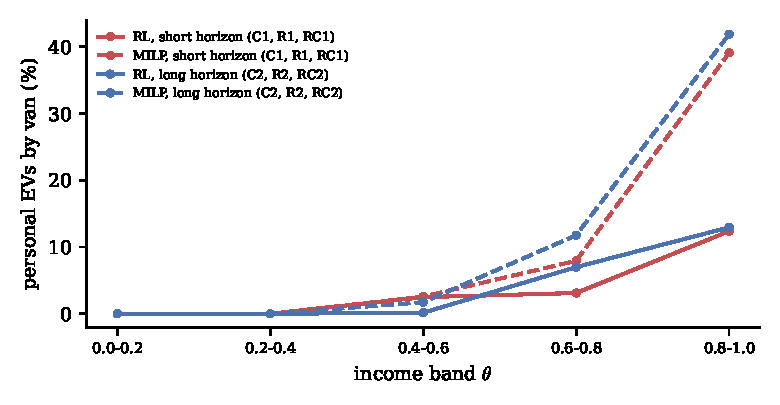
\includegraphics[width=0.6\textwidth]{figures/r_horizon.pdf}
\caption{Van share of personal free-choice EVs by income band, short against long horizon, RL (solid) and MILP (dashed).}
\label{fig:horizon}
\end{figure}

\begin{table}[H]\centering
\small
\caption{Van share (\%) of free-choice EVs by family and segment, RL against MILP.}\label{tab:families}
\begin{adjustbox}{max width=\textwidth}\begin{tabular}{llrrrrrr}\toprule
family & horizon & free-choice EVs & mean pressure & pers. by van RL & pers. MILP & comm. by van RL & comm. MILP \\ \midrule
C1 & short & 4\,104 & 0.38 & 4.7 & 21.5 & 1.1 & 0.9 \\
C2 & long & 3\,771 & 0.29 & 9.4 & 21.8 & 0.8 & 0.6 \\
R1 & short & 3\,492 & 0.82 & 5.0 & 11.8 & 0.6 & 0.2 \\
R2 & long & 5\,082 & 0.56 & 3.4 & 18.9 & 1.6 & 1.3 \\
RC1 & short & 2\,016 & 0.86 & 9.4 & 18.2 & 0.8 & 0.5 \\
RC2 & long & 3\,680 & 0.46 & 11.3 & 25.8 & 0.5 & 0.3 \\
\bottomrule\end{tabular}\end{adjustbox}\end{table}


RL's richest personal band gets a van \VanTopShort\pct{} of the time with a short horizon and \VanTopLong\pct{} with a long one. Short horizons have higher demand pressure (\PressShort{} against \PressLong).

\inshort{The horizon matters through congestion and the vans' time budget; RL's van shares stay below the MILP's in every family.}

\subsection{Infrastructure utilisation}
\label{sec:util}

All numbers in this section come from \code{common/infra.py} applied to the plans. Gun utilisation is the share of $[0,T]$ a gun is charging; at constant power this is also the share of its energy capacity used. For a van it covers seats, battery, time on the road and charging time. RL and MILP are compared on the \UtilPaired{} instances where both have a valid plan.

\subsubsection{Stations and guns}
\begin{table}[H]\centering
\caption{Infrastructure utilisation (\code{infra.utilisation}): stations, guns and the system. Paired = instances where both RL and MILP have a valid plan.}\label{tab:utilsystem}
\begin{adjustbox}{max width=\textwidth}\begin{tabular}{lrrr}\toprule
measure & RL, all valid & RL, paired & MILP, paired \\ \midrule
instances (valid plans) & 500 & 474 & 474 \\
energy asked per instance (kWh) & 1021 & 987 & 987 \\
charged at stations (\% of kWh) & 83.4 & 83.5 & 80.3 \\
gun time = energy utilisation over $[0,T]$ (\%) & 15.80 & 13.31 & 12.82 \\
idle guns per instance (of 24) & 5.8 & 6.1 & 7.0 \\
guns without any EV (\% of guns) & 24.2 & 25.6 & 29.0 \\
busiest gun (\% of $T$) & 97.6 & 92.4 & 91.4 \\
station utilisation, 90th pct (\%) & 46.5 & 34.5 & 33.4 \\
peak concurrent guns (mean) & 13.6 & 13.1 & 12.9 \\
peak concurrent guns (max) & 24 & 24 & 24 \\
installed-capacity utilisation (\%) & 14.73 & 12.39 & 12.39 \\
van fleet use (dispatched / 5, \%) & 44.2 & 41.6 & 43.9 \\
vans per instance & 2.21 & 2.08 & 2.19 \\
peak concurrent vans (mean) & 2.1 & 2.0 & 2.2 \\
\bottomrule\end{tabular}\end{adjustbox}\end{table}


\begin{figure}[H]
\centering
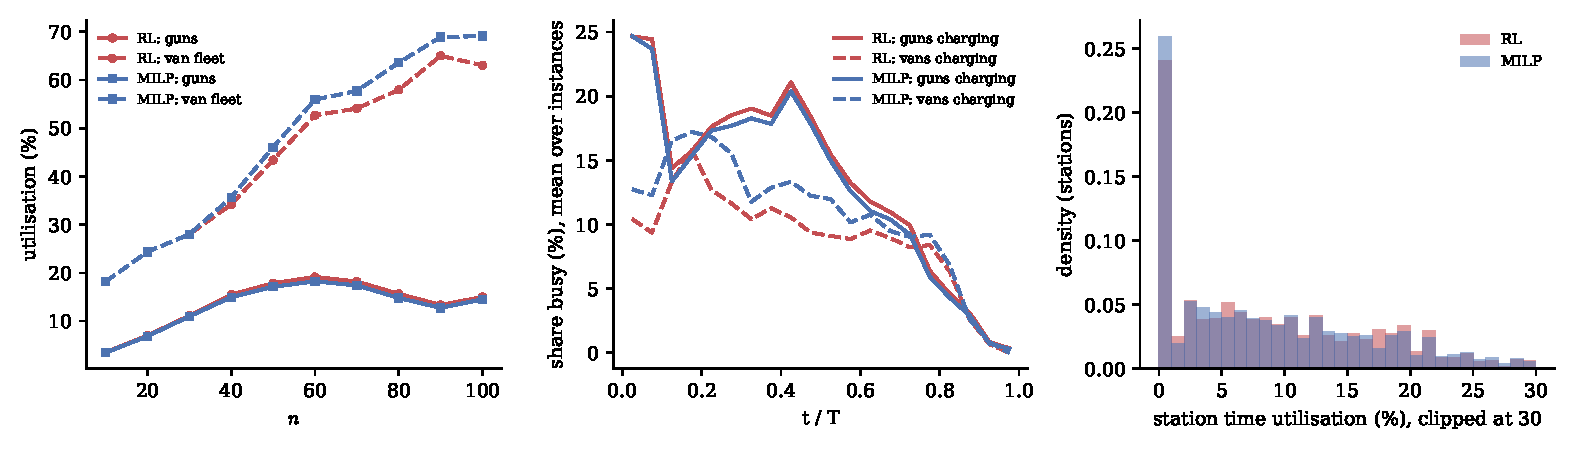
\includegraphics[width=\textwidth]{figures/r_util.pdf}
\caption{Left: gun utilisation and van fleet use by instance size. Middle: share of guns (solid) and vans (dashed) charging over the planning period, mean over the paired instances. Right: distribution of station utilisation (paired instances).}
\label{fig:util}
\end{figure}

\begin{table}[H]\centering
\small
\caption{Utilisation by family on the paired instances (\%; idle guns of 24).}\label{tab:utilfamily}
\begin{adjustbox}{max width=\textwidth}\begin{tabular}{lrrrrrrrrrrr}\toprule
family & paired & gun util RL & MILP & idle guns RL & MILP & fleet use RL & MILP & seats RL & MILP & on road RL & MILP \\ \midrule
C1 & 89 & 8.45 & 8.05 & 8.6 & 9.4 & 42.5 & 43.6 & 79.6 & 94.6 & 68.2 & 65.4 \\
C2 & 79 & 3.09 & 2.97 & 6.8 & 8.3 & 36.2 & 38.0 & 78.2 & 92.1 & 66.2 & 63.1 \\
R1 & 75 & 27.66 & 26.87 & 5.5 & 5.7 & 44.8 & 46.7 & 45.9 & 50.6 & 84.4 & 86.9 \\
R2 & 110 & 9.59 & 9.20 & 3.8 & 4.9 & 40.4 & 41.8 & 80.6 & 93.8 & 62.2 & 62.0 \\
RC1 & 42 & 31.42 & 29.96 & 6.1 & 6.3 & 41.0 & 48.6 & 37.2 & 41.3 & 84.1 & 85.3 \\
RC2 & 79 & 10.96 & 10.65 & 6.5 & 7.4 & 44.8 & 47.8 & 75.2 & 81.0 & 56.5 & 57.3 \\
\bottomrule\end{tabular}\end{adjustbox}\end{table}


\begin{itemize}
  \item \textbf{Stations are lightly used.} An average instance asks for \UtilKwhInst{} kWh. A gun is busy \UtilGunR\pct{} of the planning period in RL plans (MILP \UtilGunM\pct), \UtilGunHundredR\pct{} at $n=100$ (MILP \UtilGunHundredM\pct). The installed capacity of 24 guns and 5 vans is used \UtilSysR\pct, the same for both methods, because every plan delivers all the energy asked.
  \item \textbf{But unevenly.} \UtilIdleGunsR{} of the 24 guns per instance never charge a car in RL plans (MILP \UtilIdleGunsM), while the busiest gun is busy \UtilGunMaxR\pct{} of $T$. Use is highest in \UtilGunTopFam{} (\UtilGunTopFamV\pct) and lowest in \UtilGunLowFam{} (\UtilGunLowFamV\pct), whose horizon is 14 times longer.
  \item \textbf{The peak is at the start.} The share of guns charging peaks at \UtilProfPeakR\pct{} near $t/T=\UtilProfPeakAt$ (MILP \UtilProfPeakM\pct): the burst of requests at time 0 (Section~\ref{sec:pressure}). At the busiest moment \UtilPeakGunsR{} guns charge at once on average (MILP \UtilPeakGunsM), and all \UtilPeakGunsMaxR{} at most.
  \item \textbf{RL leans on the stations.} It charges \UtilFcsShareR\pct{} of the energy at stations (MILP \UtilFcsShareM\pct), so its guns are busier and fewer stay idle. Low average utilisation and binding gun-minutes go together: the guns are scarce only at the peak and near the clusters of requests (Section~\ref{sec:duals}).
\end{itemize}

\subsubsection{Vans}
\begin{table}[H]\centering
\caption{Use of the dispatched vans (\code{infra.utilisation}); means over vans.}\label{tab:utilvans}
\begin{adjustbox}{max width=\textwidth}\begin{tabular}{lrrr}\toprule
measure (per dispatched van) & RL, all valid & RL, paired & MILP, paired \\ \midrule
vans dispatched & 1\,105 & 985 & 1\,040 \\
seats used (\% of 6) & 67.9 & 69.4 & 79.0 \\
battery drawn (\% of 150 kWh) & 62.2 & 63.5 & 71.1 \\
on the road (\% of $T$) & 70.7 & 68.6 & 68.4 \\
charging = power-capacity use (\% of $T$) & 24.8 & 22.0 & 24.8 \\
driving (\% of $T$) & 19.7 & 17.8 & 17.9 \\
idle on the road (\% of $T$) & 26.2 & 28.8 & 25.8 \\
idle (\% of on-road time) & 37.8 & 41.6 & 38.2 \\
kWh delivered per van & 76.7 & 78.2 & 88.7 \\
energy drawn: delivered (\%) & 82.2 & 82.2 & 83.2 \\
energy drawn: transfer loss (\%) & 9.1 & 9.1 & 9.2 \\
energy drawn: driving (\%) & 8.6 & 8.7 & 7.6 \\
\bottomrule\end{tabular}\end{adjustbox}\end{table}

\begin{table}[H]\centering
\caption{What limits the dispatched vans, on the paired instances (both methods valid).}\label{tab:vans}
\begin{adjustbox}{max width=\textwidth}\begin{tabular}{lrr}\toprule
measure & RL & MILP \\ \midrule
vans dispatched (paired instances) & 985 & 1\,040 \\
stops per van (mean) & 4.16 & 4.74 \\
vans full (6 EVs, \%) & 19.4 & 48.1 \\
battery above 90\% of $B$ (\%) & 14.5 & 22.2 \\
back after 90\% of $T$ (\%) & 14.5 & 16.1 \\
seats taken by stranded EVs (\%) & 88.0 & 73.3 \\
vans serving only stranded EVs (\%) & 66.5 & 29.1 \\
tightest: seats (\%) & 41.5 & 60.4 \\
tightest: battery (\%) & 14.2 & 10.1 \\
tightest: time (\%) & 44.3 & 29.5 \\
\bottomrule\end{tabular}\end{adjustbox}\end{table}

\begin{table}[H]\centering
\small
\caption{RL van use by family, with the MILP's van count and stops for comparison.}\label{tab:vansfamily}
\begin{adjustbox}{max width=\textwidth}\begin{tabular}{lrrrrrrr}\toprule
family & vans RL & stops/van & back (\% of $T$) & tightest seats (\%) & tightest time (\%) & vans MILP & stops/van MILP \\ \midrule
C1 & 189 & 4.78 & 69.0 & 70.4 & 27.0 & 194 & 5.68 \\
C2 & 143 & 4.69 & 75.1 & 24.5 & 34.3 & 150 & 5.53 \\
R1 & 168 & 2.76 & 87.5 & 0.0 & 100.0 & 175 & 3.03 \\
R2 & 222 & 4.84 & 64.8 & 72.1 & 26.1 & 230 & 5.63 \\
RC1 & 86 & 2.23 & 88.8 & 0.0 & 100.0 & 102 & 2.48 \\
RC2 & 177 & 4.51 & 57.8 & 45.8 & 13.6 & 189 & 4.86 \\
\bottomrule\end{tabular}\end{adjustbox}\end{table}


\begin{figure}[H]
\centering
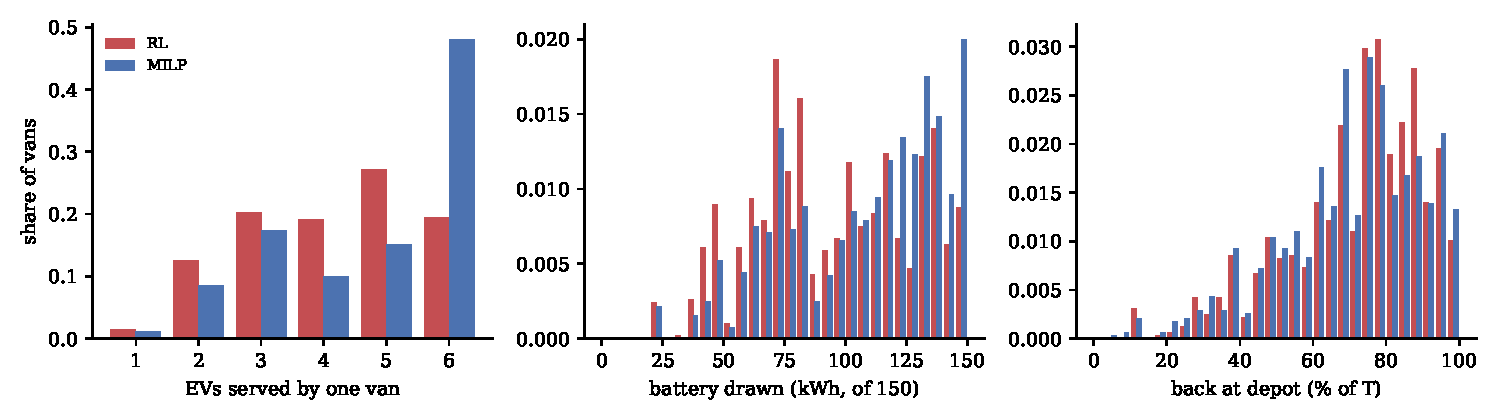
\includegraphics[width=0.95\textwidth]{figures/r_vans.pdf}
\caption{EVs per van, battery drawn and return time of every dispatched van, RL against MILP (paired instances).}
\label{fig:vans}
\end{figure}

\begin{itemize}
  \item \textbf{Fleet.} On the paired instances RL dispatches \VansR{} vans (MILP \VansM), \UtilFleetR\pct{} of the fleet on average (MILP \UtilFleetM\pct). RL does not send out more vans; it sends them out emptier.
  \item \textbf{Seats and energy.} RL vans use \UtilSeatR\pct{} of their seats (MILP \UtilSeatM\pct) and deliver \UtilVanKwhR{} kWh each (MILP \UtilVanKwhM); only \VansFullR\pct{} are full against \VansFullM\pct. In total RL vans deliver \UtilVanKwhTotR{} kWh against \UtilVanKwhTotM. \StrandedSeatsR\pct{} of RL van seats hold stranded EVs (MILP \StrandedSeatsM\pct), and \OnlyStrandedR\pct{} of RL vans serve only stranded EVs (MILP \OnlyStrandedM\pct).
  \item \textbf{Battery.} RL vans draw \UtilBattR\pct{} of their 150 kWh (MILP \UtilBattM\pct). Of the energy drawn, \UtilLossShareR\pct{} is lost in the transfer to the car and \UtilDriveShareR\pct{} is spent driving (MILP \UtilDriveShareM\pct); the rest is delivered.
  \item \textbf{Time.} A van is on the road \UtilRoadR\pct{} of $T$ (MILP \UtilRoadM\pct) but charges only \UtilChargeR\pct{} of $T$ (MILP \UtilChargeM\pct). This is its use of power capacity. \UtilIdleR\pct{} of its time on the road is idle (MILP \UtilIdleM\pct): it waits at a car for the request time, or between stops.
  \item \textbf{What limits a van.} For RL vans the tightest resource is time for \TightTimeR\pct, seats for \TightSeatsR\pct{} and the battery for \TightBattR\pct. In R1 and RC1 every van runs out of time, whatever the method.
\end{itemize}

\inshort{Both methods leave most of the installed capacity unused: guns are scarce only at the peak, and many guns stay idle. RL uses the stations a little more and the vans a little less. It dispatches about as many vans as the MILP, but fills them mainly with stranded cars, so they carry fewer customers and less energy, and spend more of their time on the road idle.}

\subsection{Money paid and perceived cost: equity}

\begin{figure}[H]
\centering
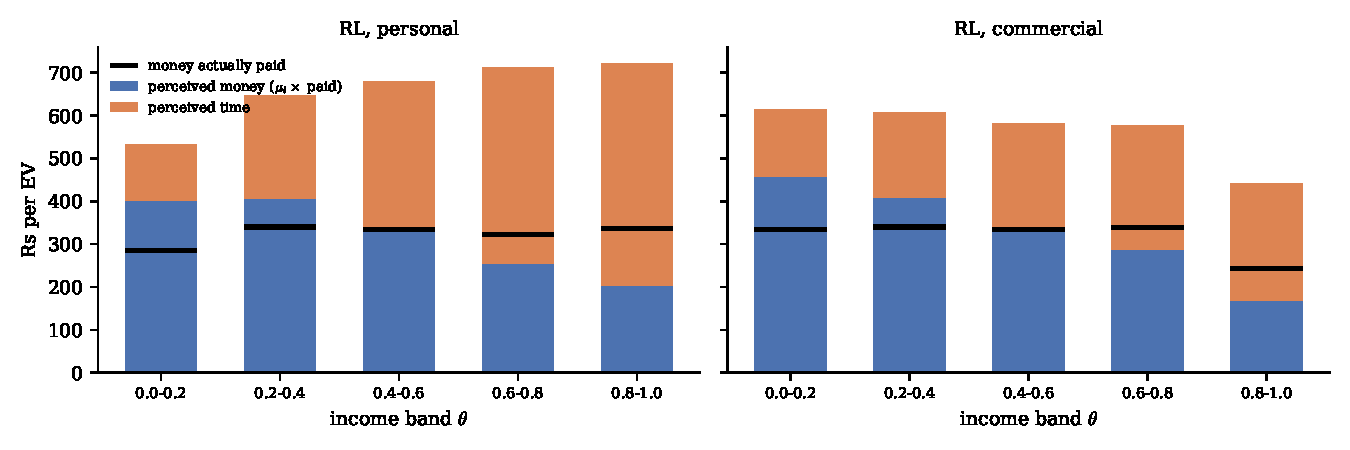
\includegraphics[width=0.9\textwidth]{figures/r_equity.pdf}
\caption{Money paid and perceived cost per EV by income band and segment (RL).}
\label{fig:equity}
\end{figure}

\begin{table}[H]\centering
\footnotesize
\caption{Money paid and perceived cost in the RL plans by segment and income band (shares of all EVs of the valid RL plans); last column: perceived cost per EV of the same group in the MILP plans.}\label{tab:equity}
\begin{adjustbox}{max width=\textwidth}\begin{tabular}{llrrrrrrrr}\toprule
segment & income $\theta$ & EVs (\%) & money paid (\%) & perceived (\%) & perceived per Rs & time share (\%) & paid per kWh & perceived/EV RL & MILP \\ \midrule
personal & 0.0--0.2 & 0.5 & 0.5 & 0.5 & 1.86 & 24.6 & 15.5 & 531 & 509 \\
 & 0.2--0.4 & 2.9 & 2.9 & 2.9 & 1.90 & 36.9 & 16.9 & 646 & 646 \\
 & 0.4--0.6 & 6.3 & 6.3 & 6.8 & 2.03 & 50.7 & 17.0 & 678 & 675 \\
 & 0.6--0.8 & 8.4 & 8.1 & 9.6 & 2.21 & 64.2 & 17.0 & 713 & 691 \\
 & 0.8--1.0 & 11.6 & 11.7 & 13.4 & 2.14 & 71.8 & 17.5 & 722 & 646 \\
commercial & 0.0--0.2 & 10.9 & 10.8 & 10.6 & 1.84 & 25.6 & 16.5 & 614 & 607 \\
 & 0.2--0.4 & 31.6 & 32.0 & 30.6 & 1.79 & 32.8 & 17.2 & 608 & 594 \\
 & 0.4--0.6 & 22.3 & 22.2 & 20.6 & 1.74 & 41.9 & 17.1 & 581 & 560 \\
 & 0.6--0.8 & 5.1 & 5.2 & 4.7 & 1.70 & 50.1 & 17.6 & 576 & 559 \\
 & 0.8--1.0 & 0.3 & 0.2 & 0.2 & 1.82 & 61.9 & 15.7 & 442 & 425 \\
\bottomrule\end{tabular}\end{adjustbox}\end{table}


\begin{itemize}
  \item A personal owner perceives \PercEvPers{} Rs per charge in RL plans (MILP \PercEvMPers). A commercial driver perceives \PercEvComm{} Rs (MILP \PercEvMComm). The extra cost of RL falls on both segments.
  \item \textbf{Perceived cost per rupee paid:} \PerRsPoorPers{} for the poorest and \PerRsRichPers{} for the richest personal band; \PerRsPoorComm{} and \PerRsRichComm{} for commercial drivers. The poor feel money strongly, the rich feel time strongly.
  \item \textbf{Price per kWh:} both segments pay about \PaidKwhPers{} Rs per kWh on average, since few get a van and pay the van tariff.
\end{itemize}

\inshort{Each group bears the cost it minds least in rupee terms. Under RL a little more of everyone's cost is waiting time.}

\subsection{Sensitivity to the segment mix}
\begin{table}[H]\centering
\caption{Expected van share of free-choice EVs for other segment mixes (reweighting of the observed segment shares; a first-order estimate).}\label{tab:mix}
\begin{adjustbox}{max width=\textwidth}\begin{tabular}{lrr}\toprule
commercial share $\pi_{\mathrm C}$ & expected van share RL (\%) & MILP (\%) \\ \midrule
0.3 & 5.0 & 14.2 \\
0.5 & 3.8 & 10.3 \\
0.7 (used) & 2.7 & 6.5 \\
0.9 & 1.5 & 2.6 \\
\bottomrule\end{tabular}\end{adjustbox}\end{table}


If the van probability of each segment stayed as observed, a market with 30\,\% commercial cars would give an expected van share of \MixRLThree\pct{} under RL (MILP \MixMThree\pct), and one with 90\,\% \MixRLNine\pct{} (MILP \MixMNine\pct). The plans would adapt, so this is a first-order estimate. The gap between the methods widens when there are more personal owners, because that is where RL departs from the MILP.

\inshort{The segment mix moves the van share strongly, and RL's under-use of vans for private owners matters more in a market with more of them.}

\subsection{Why RL behaves this way}
\begin{enumerate}
  \item \textbf{The dispatch cost comes first.} When the policy decides car by car, the first car put on a van carries the whole dispatch cost of Rs~1\,500. The next five cars on the same van come almost free. The MILP sees the whole route at once. For a policy that decides one car at a time, opening a van for a free-choice customer looks expensive, so it opens vans for stranded cars and keeps free-choice customers at stations.
  \item \textbf{Filling a van needs a coordinated series of choices} (route order, timing of the stranded stops). Random sampling during training rarely finds these, so the spare seats stay empty (\OnlyStrandedR\pct{} of vans serve only stranded cars).
  \item \textbf{Its teacher prefers stations.} The warm-up copies the greedy rule, which gives every car its cheapest option at that moment, usually a station.
  \item \textbf{The cost is flat around the best plan.} For a rich private owner the van's advantages (no drive, faster charging, driver free) and its disadvantages (van premium, dearer van energy, dispatch cost) nearly balance. So moving such a customer to a station costs little, and training receives a weak signal to do otherwise.
\end{enumerate}

\inshort{RL finds a plan almost as cheap as the MILP's with a different structure: fewer vans for free-choice customers and longer queues. This shows that many quite different plans are nearly equally good.}

\subsection{Robustness and caveats}
\begin{itemize}
  \item \textbf{One trained model, one seed.} Results come from one training run (best epoch \BestEpoch). Another seed would give somewhat different van shares.
  \item \textbf{Benchmark not always optimal.} The MILP plans of large instances are time-limit plans; gaps to them understate RL's distance from the optimum on those instances and explain the cases where RL is cheaper.
  \item \textbf{Placeholder parameters.} Directions come from the formulation, sizes from the parameter values (Table~\ref{tab:params}).
  \item \textbf{Shadow prices hold for the given decisions.} Discrete changes (one more van, seat or gun) need re-solving.
  \item \textbf{Demand pressure is a proxy:} it ignores travel time, charging still in progress and counts a van as one charger; the policy does not use it.
  \item \textbf{Invalid plans.} The \InvalidNoPlan{} open instances remain unresolved; neither method proves whether a plan exists.
\end{itemize}

%=====================================================================
\section{Summary of findings}
\begin{enumerate}
  \item RL gives a valid plan in \NValid{} of \NInst{} instances, more than the MILP (\NValidM), and fails only where the MILP fails too; most failures are infeasible data.
  \item Its plans cost \GapMean\pct{} more than the MILP's on average and \GapOpt\pct{} more than proven optima, in \RLtime\,s per instance instead of \MILPtime\,s.
  \item It improves on the greedy rule it learned from by \GreedyGapAbs\pct{} on average.
  \item The extra cost is customer waiting time. RL uses vans mainly for stranded cars and keeps rich private owners at stations: \VanRPers\pct{} of personal free-choice cars get a van, against \VanMPers\pct{} in the MILP.
  \item The behaviour predicted by formulation 4 survives in weaker form: vans for rich personal owners, almost none for taxis except at peak demand, and queues borne by low-income commercial drivers.
  \item Shadow prices show more congestion at the guns (\GunBindR\pct{} of links binding against \GunBindM\pct) and a higher value of faster guns; patience limits and the deadline have zero marginal value, as for the MILP.
  \item Infrastructure is lightly used by both methods (guns busy \UtilGunR\pct{} of $T$ in RL plans, MILP \UtilGunM\pct); RL charges more energy at stations and fills its vans less (\UtilSeatR\pct{} of seats against \UtilSeatM\pct).
  \item Opening and filling vans is the policy's weak point; a decoder that plans whole van routes, or a reward that credits a van's later passengers, is the natural improvement.
\end{enumerate}

{\footnotesize Generated from \code{2026-11-22\_formulation\_4/baseline\_RL} (results and model) and \code{baseline\_MILP/results} by \code{compute\_duals\_rl\_f4.py} and \code{make\_rl\_report.py} in this folder.}

\end{document}
